%definira klasu dokumenta 
\documentclass[12pt]{report} 

%prostor izmedu naredbi \documentclass i \begin{document} se zove uvod. U njemu se nalaze naredbe koje se odnose na cijeli dokument

%osnovni LaTex ne može riješiti sve probleme, pa se koriste različiti paketi koji olakšavaju izradu željenog dokumenta
\usepackage[croatian]{babel} 
\usepackage{amssymb}
\usepackage{amsmath}
\usepackage{txfonts}
\usepackage{mathdots}
\usepackage{titlesec}
\usepackage{array}
\usepackage{lastpage}
\usepackage{etoolbox}
\usepackage{tabularray}
\usepackage{color, colortbl}
\usepackage{adjustbox}
\usepackage{geometry}
\usepackage[classicReIm]{kpfonts}
\usepackage{hyperref}
\usepackage{fancyhdr}

\usepackage{float}
\usepackage{setspace}
\restylefloat{table}


\patchcmd{\chapter}{\thispagestyle{plain}}{\thispagestyle{fancy}}{}{} %redefiniranje stila stranice u paketu fancyhdr

%oblik naslova poglavlja
\titleformat{\chapter}{\normalfont\huge\bfseries}{\thechapter.}{20pt}{\Huge}
\titlespacing{\chapter}{0pt}{0pt}{40pt}


\linespread{1.3} %razmak između redaka

\geometry{a4paper, left=1in, top=1in,}  %oblik stranice

\hypersetup{ colorlinks, citecolor=black, filecolor=black, linkcolor=black,	urlcolor=black }   %izgled poveznice


%prored smanjen između redaka u nabrajanjima i popisima
\newenvironment{packed_enum}{
	\begin{enumerate}
		\setlength{\itemsep}{0pt}
		\setlength{\parskip}{0pt}
		\setlength{\parsep}{0pt}
	}{\end{enumerate}}

\newenvironment{packed_item}{
	\begin{itemize}
		\setlength{\itemsep}{0pt}
		\setlength{\parskip}{0pt}
		\setlength{\parsep}{0pt}
	}{\end{itemize}}




%boja za privatni i udaljeni kljuc u tablicama
\definecolor{LightBlue}{rgb}{0.9,0.9,1}
\definecolor{LightGreen}{rgb}{0.9,1,0.9}

%Promjena teksta za dugačke tablice
\DefTblrTemplate{contfoot-text}{normal}{Nastavljeno na idućoj stranici}
\SetTblrTemplate{contfoot-text}{normal}
\DefTblrTemplate{conthead-text}{normal}{(Nastavljeno)}
\SetTblrTemplate{conthead-text}{normal}
\DefTblrTemplate{middlehead,lasthead}{normal}{Nastavljeno od prethodne stranice}
\SetTblrTemplate{middlehead,lasthead}{normal}

%podesavanje zaglavlja i podnožja

\pagestyle{fancy}
\lhead{Programsko inženjerstvo}
\rhead{$Group \ Fitness \ Planer$}
\lfoot{$DevUps$}
\cfoot{stranica \thepage/\pageref{LastPage}}
\rfoot{\today}
\renewcommand{\headrulewidth}{0.2pt}
\renewcommand{\footrulewidth}{0.2pt}


\begin{document} 
	
	
	
	\begin{titlepage}
		\begin{center}
			\vspace*{\stretch{1.0}} %u kombinaciji s ostalim \vspace naredbama definira razmak između redaka teksta
			\LARGE Programsko inženjerstvo\\
			\large Ak. god. 2022./2023.\\
			
			\vspace*{\stretch{3.0}}
			
			\huge $$Group \ Fitness \ Planner$$\\
			\Large Dokumentacija, Rev. \textit{$<$1$>$}\\
			
			\vspace*{\stretch{12.0}}
			\normalsize
			Grupa: \textit{$$DevUps$$}\\
			Voditelj: \textit{$$Tomislav \ Kožul$$}\\
			
			
			\vspace*{\stretch{1.0}}
			Datum predaje: \textit{16. 11. 2022.}\\
	
			\vspace*{\stretch{4.0}}
			
			Nastavnik: \textit{Ivana Lulić}\\
		
		\end{center}

	
	\end{titlepage}

	
	\tableofcontents


	\chapter{Dnevnik promjena dokumentacije}
		
		\begin{longtblr}[
				label=none
			]{
				width = \textwidth, 
				colspec={|X[2]|X[10]|X[6]|X[3]|}, 
				rowhead = 1
			}
			\hline
			\textbf{Rev.}	& \textbf{Opis promjene/dodatka} & \textbf{Autori} & \textbf{Datum}\\[3pt] \hline
		0.1 & Opis projektnog zadatka & Tomislav Kožul  & 5.11.2022. 		\\[3pt] \hline 
  		0.2	& Dodavanje funkcionalnih i nefunkcionalnih zahtjeva  & Nika Šljubura &               5.11.2022. 	\\[3pt] \hline 
			0.3	& Dodane tablice i opisi baze podataka  & Damir Numić-Meša, Bruna Kaštela & 3.11.2022. 	\\[3pt] \hline    
			0.3.1	& Izmjena tablica baze podataka.\newline Dopisan dio ostalih zahtjeva.  & Damir Numić-Meša & 7.11.2022. 	\\[3pt] \hline 
			0.4 & Opisi obrazaca uporabe & Bruna Kaštela, Damir Numić-Meša & 10.11.2022. \\[3pt] \hline 
			0.5 & Vođenje i dodavanje dnevnika & Rujana Perić & 10.11.2022. \\[3pt] \hline 
			0.6 & Arhitektura i dizajn sustava. \newline Dijagrami razreda. & Damir Numić-Meša & 14.11.2022. \\[3pt] \hline 
			0.6.1 & Popravljeni dijagrami razreda. \newline Dijagram baze podataka. & Damir Numić-Meša & 15.11.2022. \\[3pt] \hline 
			0.7 & Specifikacija programske potpore & Nika Šljubura & 5.11.2022\\[3pt] \hline 
			0.8 & Izmjena opisa projektnog zadatka & Tomislav Kožul & 16.11.2022\\[3pt] \hline 
            0.9 & Dodani sekvencijski dijagrami & Rujana Perić & 18.11.2022\\[3pt] \hline
            0.9 & Dodani dijagrami obrasca uporabe & Petra Renić & 18.11.2022\\[3pt] \hline
			\textbf{1.0} & \textbf{Verzija samo s bitnim dijelovima za 1. ciklus} & Rujana Perić, Bruna Kaštela & 18.11.2022. \\[3pt] \hline 
            1.1 & Dodani dijagrami aktivnosti i komponenti & Rujana Perić & 6.1.2023. \\[3pt] \hline
            1.2	& Ispravci dijagrama razreda  & Damir Numić-Meša & 5.1.2023. 	\\[3pt] \hline  
            1.3	& Dodan dijagram razmještaja, opisivanje implementacija i korištenih alata  & Damir Numić-Meša & 6.1.2023. 	\\[3pt] \hline  
            1.4	& Dodani testovi komponenti i odgovarjući opisi  & Damir Numić-Meša & 9.1.2023. 	\\[3pt] \hline
				1.5	& Dodan dijagram stanja i opis dijagrama  & Bruna Kaštela & 10.1.2023. 	\\[3pt] \hline
            1.6	& Dodan pregled konkurentskih rješenja i analiza tržišta  & Rujana Perić & 10.1.2023. 	\\[3pt] \hline
            1.7	& Dodani Selenium testovi sustava  & Damir Numić-Meša & 11.1.2023. 	\\[3pt] \hline 
            1.8	& Dodane upute za puštanje aplikacije u pogon  & Rujana Perić & 11.1.2023. 	\\[3pt] \hline 
            1.9 & Dodan zaključak & Rujana Perić & 12.1.2023. 	\\[3pt] \hline 
            

			\end{longtblr}
	
	
\chapter{Opis projektnog zadatka}
		
		{Cilj ovog projektnog zadatka je napraviti web aplikaciju koja polaznicima treninga omogućuje rezervaciju odgovarajućeg termina treninga i postavljanje osobnih ciljeva koje žele ostvariti u nadolazećem mjesecu, a terenima daje mogućnost planiranja i treninga ovisno prema ciljevima korisnika i daje im mogućnosti postavljanja ograničenja za treninge.\\}
		
		
		{Potreba za razvojem ovakve aplikacije iz klijentske perspektive javlja se zbog velikog broja obaveza i nemogućnosti praćenja fiksnog rasporeda treninga. Kako korisnici ne mogu pohađati svaki trening, javlja se nezadovoljstvo iz dva razloga:}
		
		\begin{packed_item}
		    \item {nemogućnost pohađanja usluge koju su platili}
		    \item {usporen napredak zbog neredovitog treniranja}
		\end{packed_item}
		
		{Kako treneri ne bi gubili klijente, nudimo im mogućnost pohađanja termina u vrijeme kada klijentima odgovara.\\}
		
		
		{U aplikaciji, postoje dvije role koje korisnik može odabrati:}
		
		\begin{packed_item}
		    \item {klijent (u daljnjem tekstu vježbač)}
		    \item {trener}
		\end{packed_item}
		
		{Pri pokretanju aplikacije, ukoliko korisnik već nema postojeći račun, mora izvršiti registraciju. Pri registraciji, korisnik mora unijeti određene podatke:}
		
		\begin{packed_item}
		    \item {ime}
		    \item {prezime}
		    \item {datum rođenja}
		    \item {email adresa}
		    \item {korisničko ime}
		    \item {kontakt broj}
		    \item {lozinka}
		    \item {tip korisnika (vježbač ili trener)}
		    \begin{packed_item}
		        \item {ako je tip vježbač, potrebno je unijeti i cilj}
		    \end{packed_item}
		\end{packed_item}
		
		{
		Lozinka koju korisnik unese mora imati 8 – 20 znakova.\\}
		
		{Pri registraciji, vježbač odabire vlastiti cilj na temelju kojeg mu trener određuje treninge. Postoje tri različita cilja koja korisnik može odabrati:}
		
		\begin{packed_item}
            \item {povećanje mišićne mase}
            \item {izdržljivost}
            \item {gubitak težine }
        \end{packed_item}
        
        % {Treninzi za svaki cilj su različiti i zbog toga postoje četiri različite vrste treninga:}
        
        % \begin{packed_item}
        %     \item {„bodyweight“ trening}
        %     \item {trening s utezima}
        %     \item {trening snage}
        %     \item {„cardio“ trening}
        % \end{packed_item}
		
		% {Tako, ukoliko vježbač želi povećati snagu, treninzi izdržljivosti usporili bi ga na putu ka tom cilju, pa mu ih trener neće dodijeliti.\\}
		
		{Kada se vježbač registrira, dobiva potvrdni mail za registraciju koji ga odvodi na stranicu za prijavu. Po dodjeli treninga vježbaču se unutar aplikacije prikazuju njemu dodijeljeni treninzi (i termini istih).\\}
		
		
		{Kada netko od trenera vježbaču dodijeli fond sati koji vježbač može iskoristiti i kada vježbač dobije ponuđene treninge, vježbač dobiva obavijest na mail te može na kalendaru odabrati termine u kojima bi htio odraditi treninge. Treninzi se odrađuju u nekoliko termina svaki radni dan:}
		
		\begin{packed_item}
            \item {8:00 sati}
            \item {10:00 sati}
            \item {12:00 sati}
            \item {14:00 sati}
            \item {16:00 sati}
            \item {18:00 sati}
            \item {20:00 sati}

        \end{packed_item}
        
        {Ako vježbač ipak ne može pohađati trening za koji se prijavio, moguće je poništiti rezervaciju bez gubitka fonda sati.\\}
        
        {Vježbač može nakon nekog vremena, ili na samom početku, izgubiti volju ili motivaciju za određenom vrstom treninga i zbog toga mu moramo omogućiti određenu fleksibilnost. Zadnji tjedan u mjesecu, vježbaču ćemo omogućiti promjenu cilja.}
        
        {Kada vježbač rezervira termin, njegov fond sati se umanjuje za duljinu trajanja treninga koja je u našem slučaju 2h. S druge strane, otkazivanjem rezervacije, njegov fond sati se uvećava za duljinu treninga, tako da rezervacija te otkaz iste nemaju utjecaj na korisnikov fond sati.\\}
		
		{Ako vježbač odluči ne doći na trening, ukoliko nije poništio rezervaciju, rezervirani trening se računa kao odrađeni, iako ga vježbač nije pohađao. Time vježbači gube mogućnost naknadnog odrađivanja rezerviranog treninga.\\}
		
		
		{Radi ograničenog broja opreme, treneri moraju definirati i maksimalan broj polaznika za određenu vrstu treninga. Kada su sva slobodna mjesta za određeni trening popunjena, termin nestaje iz aplikacije i korisnici ga više ne mogu vidjeti.\\}
		
		{Treneri trebaju napraviti raspored treninga prema određenim ciljevima vježbača kako bi vježbači mogli što prije ispuniti svoje ciljeve i biti zadovoljni pruženom uslugom.\\}
		
		{Kao primjer, uzmimo vježbača koji želi povećati izdržljivost. Trener u skladu s ciljem vježbača treba uzeti u obzir fond sati koji bi odgovarali za postizanje navedenog cilja te na temelju oba faktora odrediti koliko različitih vrsta treninga vježbač treba odraditi.\\}
		
		
		{Iako više treninga može biti "tipa" trening snage (što će često biti vidljivo u nazivu treninga), to ne znači da svi treninzi istog ili sličnog naziva nužno sadrže iste vježbe. Treneru je dano na vlastitu prosudbu da pri izradi treninga definira koje vježbe isti obuhvaća. \\}


        {Za vježbače postoji ograničenje na broj mogućih rezervacija termina treninga tjedno. Ograničenje je skalirano prema fondu sati koje je vježbaču dodijeli trener, tj. vježbači sa velikim fondom sati imaju mogućnost većeg broja rezervacija tjedno u odnosu na manji fond sati. \\}
		
        
        {Ako vježbač pokuša prekršiti ograničenje broja mogućih rezervacija, aplikacija ga o tome obavijesti porukom i ne dopušta mu izvršavanje rezervacije koja krši zadano pravilo.\\}
        
        {Uz unaprijed definirano pravilo koje provjerava aplikacija, treneri mogu pri izradi treninga napisati vlastita pravila (u sklopu opisa treninga).\\}
        
        {Administrator je uloga koja ima mogućnosti upravljanja korisničkim računima (brisanje računa) te verifikaciju trenera.\\
        Pri registraciji, korisnik odabire ulogu trenera ili vježbača. Kako se bilo tko ne bi mogao neovlašteno registrirati kao trener, administrator mora potvrditi (verificirati) registraciju trenera.\\
        Nema mogućnost mijenjati raspored ili program koji su treneri definirali.\\}

        
        {Aplikacija je dostupna na "\href{https://group-fitness-planer-q3fc.onrender.com}{Group Fitness Planner.}"}
		\eject

        \section{Pregled konkurentskih rješenja i analiza tržišta\\}

        {Istražujući na internetu, naišli smo na nekolicinu aplikacija sa sličnim namjenama kao što je i naša. Kako se teži digitalizaciji i navika ljudi je glavninu informacija o onome što ih zanima pronaći na internetu, tako i razna poduzeća teže imati kompletnu i interaktivnu internetsku uslugu preko koje se reklamiraju, organiziraju, a ponekad i djeluju raznim on-line sadržajima. \\ \\ }
        {Primjerice, servis Exercise (\href{https://www.exercise.com}{https://www.exercise.com/}) nudi jedinstvenu platformu za upravljanje fitness ustanovom, od mogućnosti registracije polaznika i pretplatnika na usluge, zaposlenika i voditelja, do registracije lokacija na kojima se odvijaju aktivnosti, e-potpisivanja ugovora i pretplata, kreiranja treninga, TV-treninga i biblioteke treninga i vježbi, statistike dolazaka na treninge, izvješća o napredovanju, online live prijenosa, izazova…}
        
              \begin{figure}[H]
                      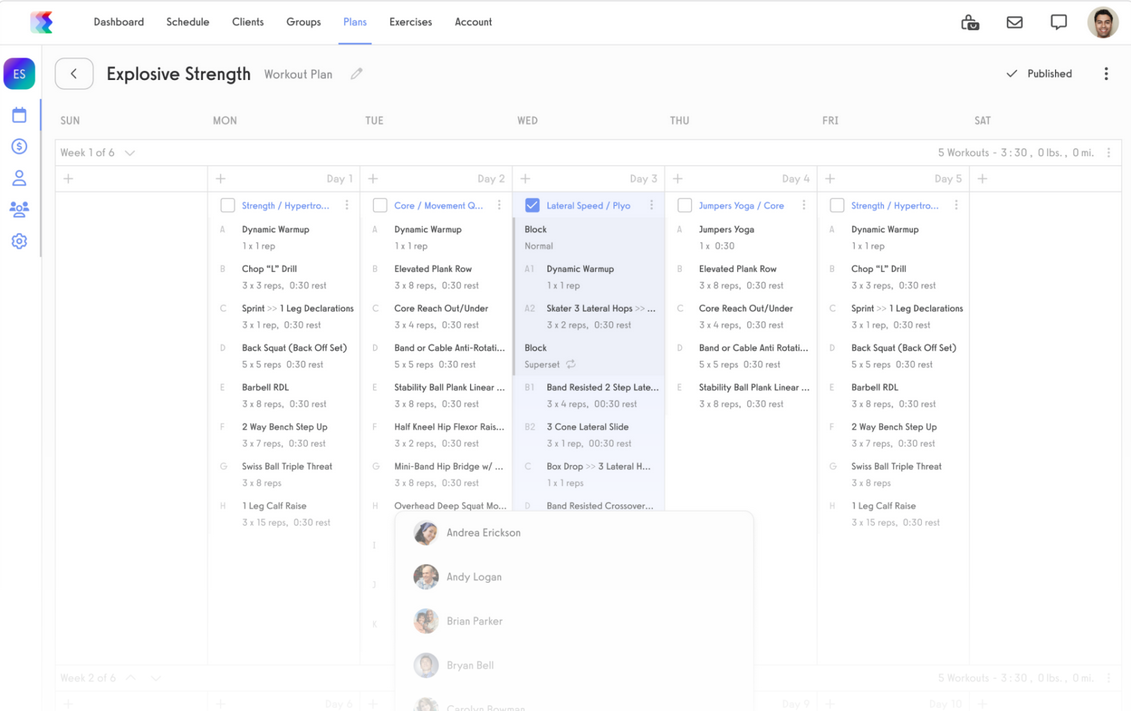
\includegraphics[scale=0.5]{./Slike/trainer_workouts.png}
                      \centering
                      \caption{Exercise}
                      \label{fig:promjene}
                \end{figure}

                \begin{figure}[H]
                      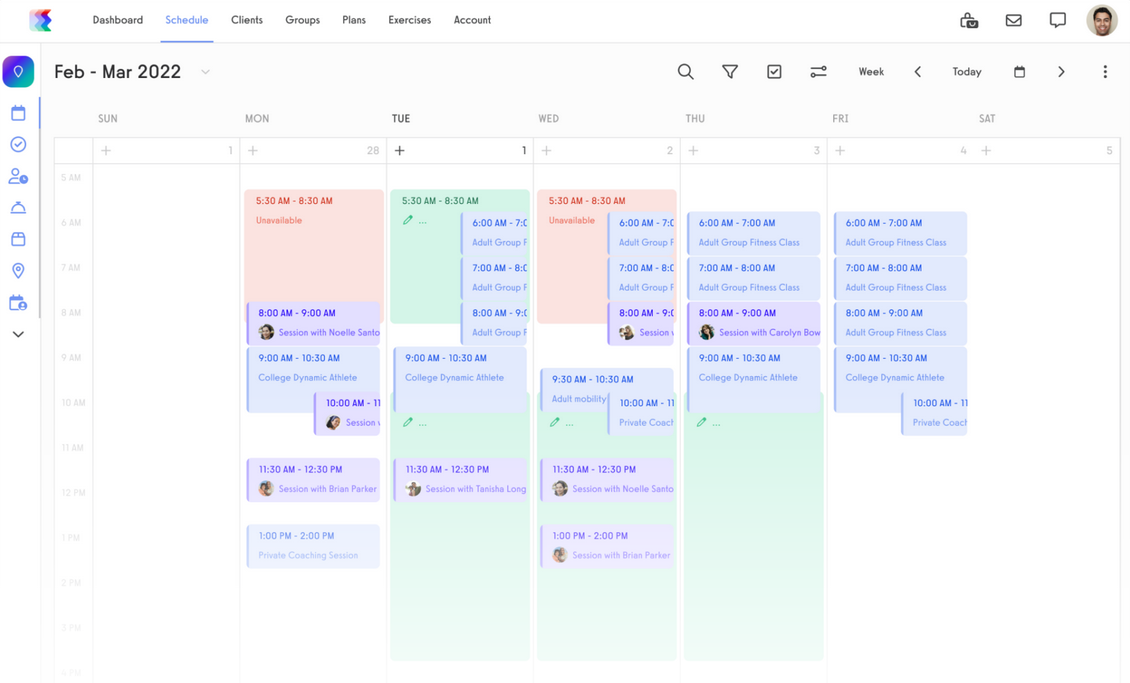
\includegraphics[scale=0.5]{./Slike/trainer_schedule.png}
                      \centering
                      \caption{Exercise}
                      \label{fig:promjene}
                \end{figure}

                \begin{figure}[H]
                      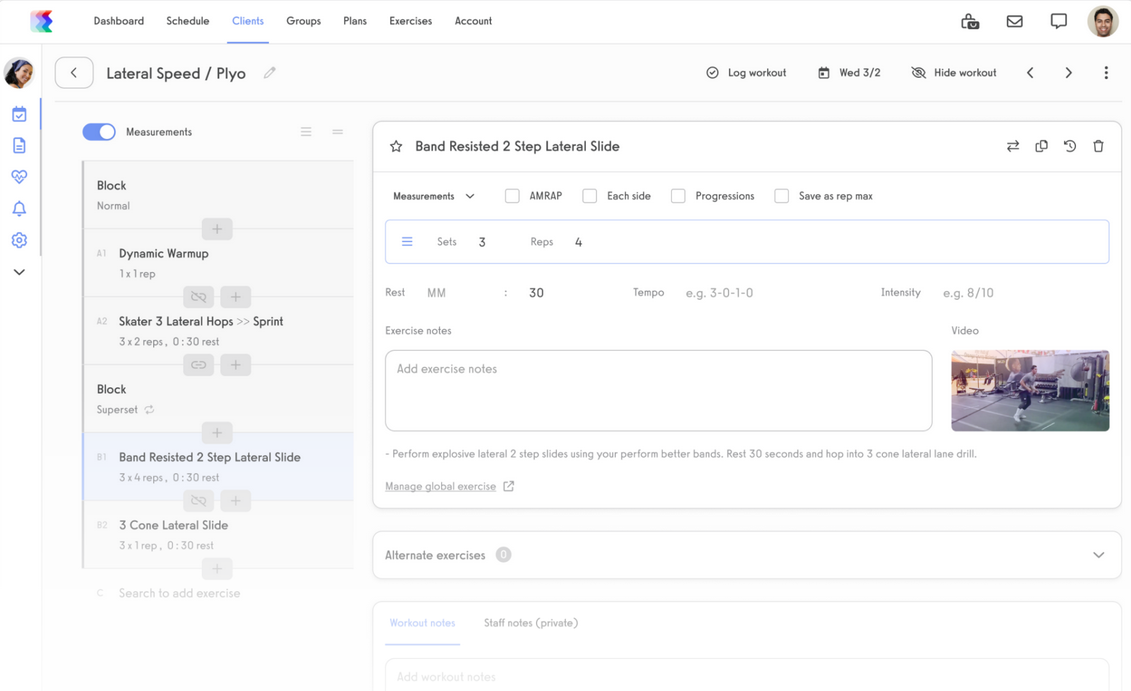
\includegraphics[scale=0.5]{./Slike/trainer_client.png}
                      \centering
                      \caption{Exercise}
                      \label{fig:promjene}
                \end{figure}

                 \begin{figure}[H]
                      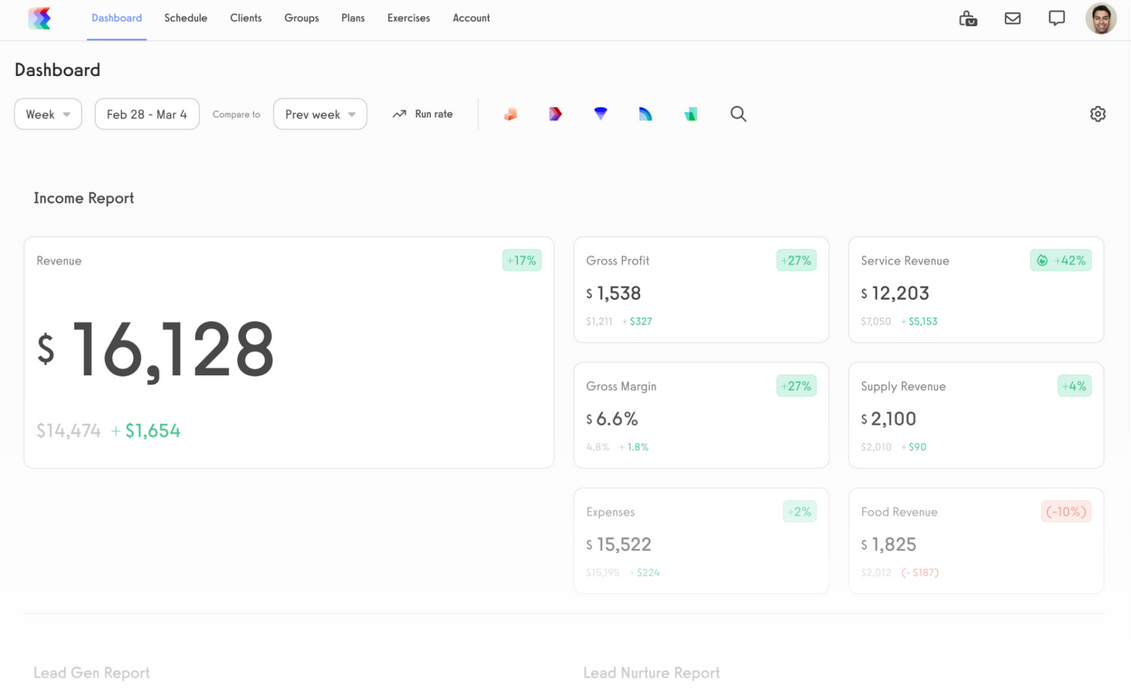
\includegraphics[scale=0.5]{./Slike/stats.png}
                      \centering
                      \caption{Exercise}
                      \label{fig:promjene}
                \end{figure}
        {Exercise obuhvaća puno veći spektar usluga nego što obuhvaća naša „Group fitness planner“ aplikacija, pa je samim time naša aplikacija namijenjena užem krugu klijenata. Ciljani klijenti su manji fitness centri sa jednim prostorom za vježbanje, koji pomoću dobre organizacije i individualiziranog pristupa treninzima žele steći povjerenje kod svojih korisnika i imati maksimalnu učinkovitost u pogledu prilagođavanja vrste i termina treninga po želji i mogućnostima svojih korisnika. Aplikacija je jednostavna i intuitivna za korištenje, te sa samo nekoliko funkcionalnosti ispunjava svrhu opisanu opisom projektnog zadatka. \\ \\}
                \begin{figure}[H]
                      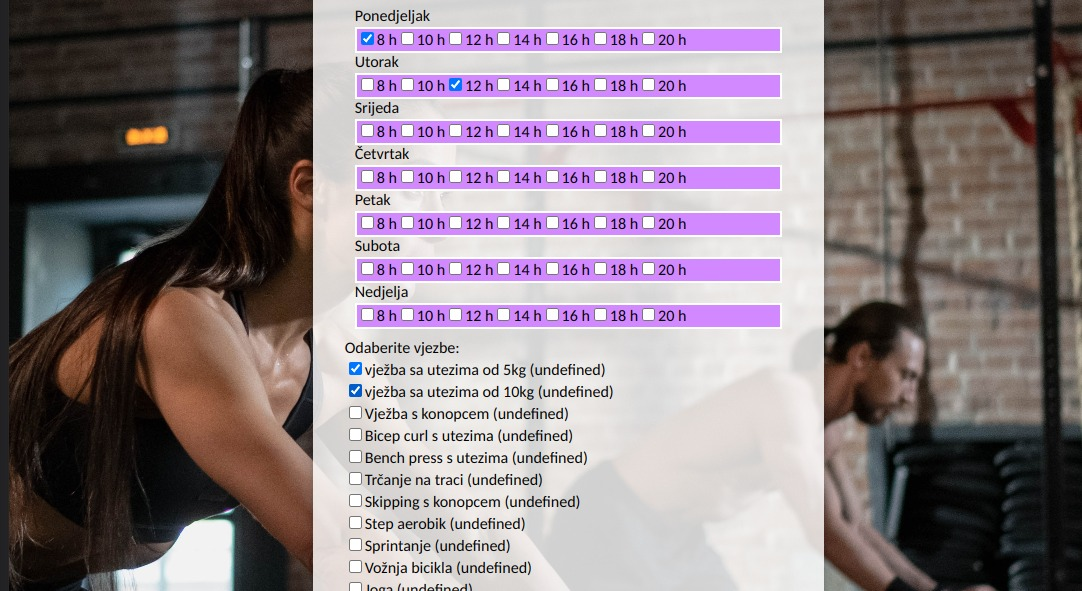
\includegraphics[scale=0.4]{./Slike/front.png}
                      \centering
                      \caption{Group fitness planner}
                      \label{fig:promjene}
                \end{figure}

        {Osim opisanog servisa Excercise, na tržištu su dostupni i sljedeći servisi: Mindbody \href{https://www.mindbodyonline.com/business/fitness-software}{(https://www.mindbodyonline.com/business/fitness-software)} aplikacija koja ima mnoge verzije, a svaka je prilagođena tipu poduzeća (za frizere, za fitness centre, za sportske klubove, za studije ljepote…) i ovisno o verziji sadržava funkcionalnosti potrebne za upravljanje tim poduzećem što intenzivno širi područja primjene aplikacije i skupinu ciljanih klijenata, Zenplanner \href{https://zenplanner.com/}{(https://zenplanner.com/)}... \\ }

        {Da bismo dobili uvid u stvarni interes potencijalnih kupaca našeg proizvoda odlučili smo kontaktirati lokalni sportski klub i postaviti trenerima i polaznicima u klubu Google forms upitnik \href{https://docs.google.com/forms/d/e/1FAIpQLSenHBNtxCLnlzAUZP_xeXSPl-oNTVsIt4iL1JYWlX9hdUSjcg/viewform?usp=sf_link}{(https://docs.google.com/forms)} .\\ }

        {Rezultati upitnika nalažu da su mišljenja oko aplikacije podijeljena. Dok su vježbači oduševljeno prihvatili osmišljeni sustav, treneri su rezerviraniji prema njemu i vide moguće nedostatke. \\Vježbači se apsolutno slažu sa idejom o plaćanju treninga po terminima (umjesto mjesečno, unaprijed), te sa mogućnošću dolaska na različite tipove treninga, koji se poklapaju sa njihovim ciljevima. \\Zanimljivo je istaknuti kako vježbači smatraju da je određivanje fitness ciljeva na mjesečnoj bazi prečesto, te se sugerira timu da u budućem radu obrati pozornost na taj podatak. }
                \begin{figure}[H]
                      
\includegraphics[scale=0.8]{./Slike/vježbači.png}
                      \centering
                      \caption{Rezultati ankete}
                      \label{fig:promjene}
                \end{figure}
                \begin{figure}[H]
                      
\includegraphics[scale=0.7]{./Slike/mjenjanjeciljeva.png}
                      \centering
                      \caption{Rezultati ankete}
                      \label{fig:promjene}
                \end{figure}
        {Također, vježbači su sugerirali da bi u ovakvoj aplikaciji voljeli vidjeti status svog napretka. Budućnost razvoja ovakve aplikacije mogla bi se usmjeriti na to, da uz postojeće funkcionalnosti, implementira i podatke o dolascima i redovitosti te napraviti stranicu sa statistikama konzistentnosti i napretka u postizanju željenih ciljeva. Također, voljeli bi imati „objašnjenja“ i neke osnovne edukativne materijale na stranici o tome koji su treninzi potrebni za koje ciljeve, koliko često se treba trenirati, koliko intenzivno… Iako smo mi na to vodili računa u implementaciji, korisnik iz korisničkog sučelja nema takav dojam, a aplikacija bi trebala biti jednostavna i intuitivna, te „voditi te“ kroz fitness iskustvo. \\}

        {Treneri su skeptični prema ovakvoj aplikaciji jer smatraju da bi kvaliteta njihovog rada bila značajno umanjena, ponajviše time što ne bi imali stalne grupe polaznika na koje mogu računati, i koje već poznaju, pa time i pomažu i prilagođavaju određene zadatke. Smatraju kako bi pod izlikom „danas mi ne odgovara dani termin, pa ću odraditi neki drugi trening“ klijenti otežavali i usporavali dostizanje određenih ciljeva. Također, smatraju da u klasičnim grupama s vremenom mogu zadavati sve teže i dinamičnije treninge, kako ljudi napreduju. Na ovakvim treninzima, uvijek bi bilo ljudi sa svim stupnjevima vještine, od početnika do iskusnih, te da bi bilo teško osmišljavati treninge takvim grupama. \\}

        {Pri razvoju svakako treba poštovati mišljenja stručnjaka i naći rješenje koje će djelomično zadovoljavati obje strane. Treneri predlažu da se treninzi, uz obzir na odabir ciljeva, dijele i prema stupnju fizičke spreme. Da stari i novi polaznici imaju svoje zasebne termine, i da sustav prepoznaje da je neki vježbač prvih mjesec-dva po registraciji „početnik“, osim ako vježbač zbog svoje prethodne sportske podloge ne zatraži drugačije. \\}
            
		\eject

        
	\chapter{Specifikacija programske potpore}
		
	\section{Funkcionalni zahtjevi}
			
		
			
			
			\noindent \textbf{Dionici:}
			
			\begin{packed_enum}
				
				\item Vježbači
				\item Treneri			
				\item Administrator
				\item Baza podataka
				
			\end{packed_enum}
			
			\noindent \textbf{Aktori i njihovi funkcionalni zahtjevi:}
			
			
			\begin{packed_enum}
				\item  \underbar{Neregistrirani/neprijavljeni korisnik može:}
				
				\begin{packed_enum}
					
					\item se registrirati u sustav, stvoriti novi korisnički račun za koji su mu potrebni korisničko ime, lozinka, ime, prezime, broj mobitela, e-mail adresa, datum rođenja, uloga, cilj (ovisno o ulozi)
				
					
				\end{packed_enum}
			
				\item  \underbar{Vježbač (primarni dionik) može:}
				
				\begin{packed_enum}
					
					\item pregledavati i mijenjati osobne podatke
					\item birati i rezervirati određenu vrstu treninga u skladu sa postavljenim ciljevima
     				\item otkazivati rezervacije
					\item odabrati željeni fitness cilj
					\item mijenjati ciljeve završetkom tekućeg mjeseca
					
				\end{packed_enum}
				
				\item  \underbar{Trener (primarni dionik) može:}
				
				\begin{packed_enum}
					
					\item određivati vrstu treninga po terminima
					\item napraviti raspored treninga prema određenim ciljevima vježbača
					\item na temelju fonda sati koji je odabrao vježbač odrediti koliko različitih vrsta treninga vježbač mora odraditi
					\item izraditi trening
					\item za vrste treninga napisati vlastita pravila
					\item definirati maksimalan broj polaznika za određenu vrstu treninga
					
				\end{packed_enum}
				
				
				\item  \underbar{Administrator (sekundarni dionik) može:}
				
				\begin{packed_enum}
					
					\item vidjeti popis svih registriranih korisnika i njihovih osobnih podataka
					\item verificirati račune trenera
					\item brisati korisničke račune
				
					
				\end{packed_enum}
				
				
				\item  \underbar{Baza podataka (sudionik) može:}
				
				\begin{packed_enum}
					
					\item pohranjuje sve podatke o korisnicima i njihovim ovlastima
					\item pohranjuje sve podatke o treninzima, vježbama, terminima i njihovim opisima i ograničenjima
				
					
				\end{packed_enum}
				
			\end{packed_enum}
			
			\eject 
			
			
				
			\subsection{Obrasci uporabe}
				
				%\textbf{\textit{dio 1. revizije}}
				
				\subsubsection{Opis obrazaca uporabe}
					
					\noindent \underbar{\textbf{UC1 - Registriraj korisnika}}
					\begin{packed_item}
	
						\item \textbf{Glavni sudionik: } Neregistrirani korisnik
						\item  \textbf{Cilj:} Izrada korisničkog računa
						\item  \textbf{Sudionici:} Baza podataka
						\item  \textbf{Preduvjet:} Pristup aplikaciji putem web preglednika
						\item  \textbf{Opis osnovnog tijeka:}
						
						\item[] \begin{packed_enum}
							
							\item Neregistrirani korisnik bira opciju "Registriraj se"
       					\item Sustav otvara formu za upis podataka
							\item Neregistrirani korisnik unosi potrebne podatke (matični i kontakt podatci)
							\item Neregistrirani korisnik odabire tip registracije (klijent ili trener)
							\begin{packed_enum}
							    \item Neregistrirani korisnik odabire tip registracije \textit{trener} i sustav preskače korak 5.
							    \item Neregistrirani korisnik odabire tip registracije \textit{klijent}
							\end{packed_enum}
							
							\item Neregistrirani korisnik odabire cilj
							
                            \item Neregistrirani korisnik odabire gumb "Registriracija"
							\item Sustav provjerava i utvrđuje dostupnost korisničkog imena i maila te ispravnost ostalih unesenih podataka u skladu s zahtjevima sustava
							\item Sustav na upisani mail šalje se link za aktivaciju korisničkog računa
                            \item Sustav pohranjuje potvrdu maila, aktivira korisnički račun i obavještava korisnika o uspješnoj registraciji
                            \item Sustav preusmjerava registriranog korisnika na stranicu "Prijava"
							
						\end{packed_enum}
						
						\item  \textbf{Opis mogućih odstupanja:}
						
						\item[] \begin{packed_item}

      					\item[6.a] Neregistrirani korisnik odustaje od registracije
							\item[] \begin{packed_enum}
								
								\item Neregistriranog se korisnika preusmjerava na početnu stranicu
								
							\end{packed_enum}
	
							\item[7.a] Sustav je provjerio i utvrdio da je neregistrirani korisnik unio neispravan oblik mail adrese, email već postoji u bazi podataka, unio je korisničko ime koje se već koristi ili je unio lozinku u nedozvoljene duljine
							\item[] \begin{packed_enum}
								
								\item Sustav obavještava neregistriranog korisnika o pogreškama te se izvođenje tijeka nastavlja u koraku 4.
								
							\end{packed_enum}

						\end{packed_item}
					\end{packed_item}
     
					\noindent \underbar{\textbf{UC2 - Prijavi korisnika}}
					\begin{packed_item}
	
						\item \textbf{Glavni sudionik: }Korisnik
						\item  \textbf{Cilj:} Prijava u sustav
						\item  \textbf{Sudionici:} Baza podataka, korisnik
						\item  \textbf{Preduvjet:} Pristup aplikaciji putem web preglednika
						\item  \textbf{Opis osnovnog tijeka:}
						
						\item[] \begin{packed_enum}
							\item Korisnik bira opciju "Prijava"  
       					\item Sustav otvara formu za upis podataka
							\item Korisnik upisuje svoje korisničko ime i lozinku
                            \item Korisnik odabire potvrdu aplikacije
							\item Sustav provjerava i utvrđuje postojanje i ispravnost podataka unesenih u formu
                            \item Sustav obavještava korisnika o uspješnoj prijavi
                            \item Sustav preusmjerava korisnika na glavnu stranicu
							\item Korisnik dobiva pristup korisničkim funkcijama ovisnima o ulozi

						\end{packed_enum}
						
						\item  \textbf{Opis mogućih odstupanja:}
						
						\item[] \begin{packed_item}
      					\item[4.a] Korisnik odustaje od prijave
       
						\item[5.a] Sustav je provjerio i utvrdio da je korisnik upisao neispravno korisničko ime i/ili lozinku ili račun nije verificiran putem maila i/ili od strane administratora (za slučaj prijave trenera)
							\item[] \begin{packed_enum}
								
								\item Sustav obavještava korisnika o pogreškama te se izvođenje tijeka nastavlja u koraku 4.					
							\end{packed_enum}
                        \end{packed_item}
                    \end{packed_item}

					\noindent \underbar{\textbf{UC3 - Odjavi korisnika}}
					\begin{packed_item}
	
						\item \textbf{Glavni sudionik: } Korisnik
						\item  \textbf{Cilj:} Odjavljivanje korisnika iz sustava
						\item  \textbf{Sudionici:} Baza podataka
						\item  \textbf{Preduvjet:} Korisnik mora biti prijavljen u sustav
						\item  \textbf{Opis osnovnog tijeka:}
						
						\item[] \begin{packed_enum}
	
							\item Prijavljeni korisnik bira opciju "Odjava"
							\item Sustav prijavljenom korisniku prikazuje prozor za potvrdu odjave
							\item Korisnik potvrđuje odjavu klikom 
							\item Sustav odjavljuje korisnika
							\item Sustav preusmjerava korisnika na stranicu za prijavu
							
						\end{packed_enum}
						\item  \textbf{Opis mogućih odstupanja:}
						
						\item[] \begin{packed_item}
	
							\item[3.a] Prijavljeni korisnik odustaje od odjave
							\item[] \begin{packed_enum}

                                \item Sustav zatvara prozor za potvrdu odjave iz sustava
								
                
								
							\end{packed_enum}
							
						\end{packed_item}
						
					\end{packed_item}
     
					\noindent \underbar{\textbf{UC4 - Pregledaj korisničke podatke}}
					\begin{packed_item}
	
						\item \textbf{Glavni sudionik: }Korisnik
						\item  \textbf{Cilj:} Pregled osobnih podataka
						\item  \textbf{Sudionici:} Baza podataka
						\item  \textbf{Preduvjet:} Korisnik je prijavljen u sustav
						\item  \textbf{Opis osnovnog tijeka:}
						
						\item[] \begin{packed_enum}
							\item Prijavljeni korisnik bira opciju ”Osobni podatci”
                            \item Sustav preusjerava prijavljenog korisnika na stranicu "Osobni podatci"
                            \item Sustav učitava iz baze podataka osobne podatke prijavljenog korisnika(matični i kontakt podatci)
                            \item Sustav prikazuje učitane podatke na stranici
                            \item Korisnik pregledava prikazane podatke
						\end{packed_enum}
                        
                    \end{packed_item}	
                    
					\noindent \underbar{\textbf{UC5 - Promijeni korisničke podatke}}
					\begin{packed_item}
	
						\item \textbf{Glavni sudionik: }Korisnik
						\item  \textbf{Cilj:} Promjena osobnih podataka
						\item  \textbf{Sudionici:} Baza podataka
						\item  \textbf{Preduvjet:} Korisnik je prijavljen u sustav
						\item  \textbf{Opis osnovnog tijeka:}
						
						\item[] \begin{packed_enum}
	
							\item Korisnik odabire opciju ”Promjena podataka”
       					\item Sustav otvara formu za promjenu podataka
                            \item Prijavljeni korisnik mijenja podatke po želji
                            \item Prijavljeni korisnik odabire potvrdu aplikacije
                            \item Sustav provjerava i utvrđuje jesu li novi podatci ispravnog oblika
                            \item Sustav pohranjuje nove podatke u bazu podataka
                            \item Sustav obavještava prijavljenog korisnika o uspješnoj promjeni                           
                            \end{packed_enum}
						
	                \item  \textbf{Opis mogućih odstupanja:}
                    \item[] \begin{packed_item}
							\item[4.a] Prijavljeni korisnik je odustao od promjene
							\item[] \begin{packed_enum}
								
								\item Sustav preusmjerava prijavljenog korisnika na stranicu "Osobni podatci"				
							\end{packed_enum}
                            \item[5.a] Sustav je utvrdio da uneseni podatci nisu ispravnog formata
							\item[] \begin{packed_enum}
								
								\item Sustav obavještava prijavljenog korisnika o pogreškama te se izvođenje tijeka nastavlja u koraku 3.					
							\end{packed_enum}
                        \end{packed_item}
                    \end{packed_item}

					\noindent \underbar{\textbf{UC6 - Obriši korisnički račun}}
					\begin{packed_item}
	                   
						\item \textbf{Glavni sudionik: } Admin
						\item  \textbf{Cilj:} Brisanje korisničkog računa iz baze podataka
						\item  \textbf{Sudionici:} Baza podataka
						\item  \textbf{Preduvjet:} Administrator mora biti prijavljen u sustav
						\item  \textbf{Opis osnovnog tijeka:}
						
						\item[] \begin{packed_enum}
	
							\item Adminstrator bira opciju "Obriši korisnički račun"
							\item Administratoru se prikazuje prozor u kojem potvrđuje brisanje korisničkog računa
                            \item Administrator odabire potvrdu aplikacije
							\item Sustav briše račun iz baze podataka
							\item Sustav obavještava administratora o uspješnom brisanju računa
							\item Sustav obavještava korisnika o brisanju računa
							
						\end{packed_enum}
						\item  \textbf{Opis mogućih odstupanja:}
						\item[] \begin{packed_item}
	
							\item[3.a] Administrator odustaje od brisanja računa
							\item[] \begin{packed_enum}

                                \item Zatvaranje prozora za potvrdu brisanja računa iz sustava

							\end{packed_enum}
							
						\end{packed_item}
      
					\end{packed_item}

					\noindent \underbar{\textbf{UC7 - Promijeni cilj}}
					\begin{packed_item}
	
						\item \textbf{Glavni sudionik: }Klijent
						\item  \textbf{Cilj:} Odabir cilja sudjelovanja u programu vježbanja
						\item  \textbf{Sudionici:} Baza podataka
						\item  \textbf{Preduvjet:} Zadnji je tjedan tekućeg mjeseca
						\item  \textbf{Opis osnovnog tijeka:}

						
						\item[] \begin{packed_enum}
	
							\item Klijent bira opciju "Promjena cilja"
							\item Sustav prikazuje klijentu ciljeve koje može odabrati
                            \item Klijent odabire cilj koji želi
							\item Klijent odabire potvrdu aplikacije
       					\item Sustav pohranjuje odabrani cilj
       					\item Sustav uklanja klijenta iz liste klijenata trenera te uklanja sve dodijeljene treninge klijentu zbog promjene cilja
       					\item Sustav obavještava klijenta o uspješnoj promjeni cilja
						\item Klijenta se preusmjerava na glavnu stranicu
							
						\end{packed_enum}
						\item  \textbf{Opis mogućih odstupanja:}
						\item[] \begin{packed_item}
	
							\item[4.a] Klijent odustaje od promjene cilja
							\item[] \begin{packed_enum}

                                \item Sustav preusmjerava klijenta na glavnu stranicu

								
							\end{packed_enum}
							
						\end{packed_item}
      
					\end{packed_item}
						

					\noindent \underbar{\textbf{UC8 - Izradi trening}}
					\begin{packed_item}
	
						\item \textbf{Glavni sudionik: }Trener
						\item  \textbf{Cilj:} Izrada treninga
						\item  \textbf{Sudionici:} Baza podataka
						\item  \textbf{Preduvjet:} Trener mora biti prijavljen u sustav
						\item  \textbf{Opis osnovnog tijeka:}
						
						\item[] \begin{packed_enum}
	
							\item Trener bira opciju "Izradi trening"
							\item Sustav otvara prozor za izradu treninga s formom za unos podataka o treningu
							\item Trener unosi glavne podatke o treningu
       					\item Trener odabire dane u tjednu u kojima bi se izvodio trening
							\item Sustav za svaki dan nudi opciju odabira slobodnog tremina
							\item Trener odabire po jedan termin za svaki odabrani dan
							\item Trener odabire opciju "Potvrdi" unutar forme
                            \item Sustav provjerava jesu li podaci ispravnog oblika
                            \item Sustav pohranjuje podatke o treningu i njegovim treminima u bazu podataka
                            \item Sustav obavještava trenera o uspješno unesenom treningu
                            \item Sustav preusmjerava trenera na stranicu svih njegovih treninga
						\end{packed_enum}
						
						\item  \textbf{Opis mogućih odstupanja:}
						
						\item[] \begin{packed_item}
	
							\item[8.a] Trener odustaje od izrade treninga
							\item[] \begin{packed_enum}
								
								\item Trenera se preusmjerava na stranicu svih njegovih treninga
								
								
							\end{packed_enum}
							\item[9.a] Sustav je utvrdio da je trener unio neispravan oblik podataka o treningu
							\item[] \begin{packed_enum}
								
								\item Sustav obavještava trenera o pogreškama te se izvođenje nastavlja od koraka 4.
								
								
							\end{packed_enum}							
							
						\end{packed_item}
					\end{packed_item}

					

					

				

				    \noindent \underbar{\textbf{UC9 - Pregledaj klijenate kojima nisu dodijeljeni treninzi }}
					\begin{packed_item}
	
						\item \textbf{Glavni sudionik: } Trener
						\item  \textbf{Cilj:} Dobiti uvid u klijente kojima nije dodijeljen trening
						\item  \textbf{Sudionici:} Baza podataka
						\item  \textbf{Preduvjet:} Trener je prijavljen u sustav
						\item  \textbf{Opis osnovnog tijeka:}
						
						\item[] \begin{packed_enum}
	                        
							\item Trener odabire opciju "Prikaži klijente bez dodijeljenog treninga"
							\item Sustav dohvaća podatke iz baze podataka o klijentima bez dodijeljenog treninga
							\item Sustav prikazuje dohvaćene podatke o klijentima na stranici
							\item Trener pregledava prikazane klijente
							
							
						\end{packed_enum}
						
					
					\end{packed_item}
    



					\noindent \underbar{\textbf{UC10 - Dodijeli treninge klijentu}}
					\begin{packed_item}
	
						\item \textbf{Glavni sudionik: }Trener
						\item  \textbf{Cilj:} Dodjela treninga klijentu
						\item  \textbf{Sudionici:} Baza podataka, klijent
						\item  \textbf{Preduvjeti:} Klijent je registriran u sustav, trener je priavljen u sustav
						\item  \textbf{Opis osnovnog tijeka:}
						
						\item[] \begin{packed_enum}
	
						\item Trener odabire klijenta sa stranice "Prikaz klijenata bez dodijeljenog treninga"
						
                            \item Treneru se za dodjelu prikazuju svi mogući treninzi sa opcijom "Dodijeli"
                            \item Trener odabire treninge za dodjelu opcijom "Dodijeli"
                            \item Trener unosi broj sati predviđenih za odrađivanje odabranih treninga klijenta na mjesečnoj bazi
						\item Trener potvrđuje dodijeljene treninge i unos odabirom opcije "Spremi"
						\item Sustav ispituje ispravnost spremljenih podataka
                            \item Sustav sprema dodijeljene treninge i broj sati u bazu podataka
                            \item Sustav obavještava trenera o uspješno dodijeljenim treninzima
                            \item Sustav obavještava klijenta o dodijeljenim treninzima putem emaila
                            
						\end{packed_enum}
						
						\item  \textbf{Opis mogućih odstupanja:}
						
						\item[] \begin{packed_item}

      						\item[6.a] Sustav je utvrdio da trener nije odabrao ni jedan trening i/ili unio broj sati
							\item[] \begin{packed_enum}
								
								\item Sustav ne sprema promjene, tj. ne evidentira klijenta kao onog kojemu su dodijeljeni treninzi te se izvođenje nastavlja u koraku 1.					
							\end{packed_enum}
	
							\item[5.a] Trener nije potvrdio dodijeljene treninge i/ili unio broj sati
							\item[] \begin{packed_enum}
								
								\item Sustav obavještava trenera o nespremljenim promjenama te se izvođenje nastavlja u koraku 1.
							\end{packed_enum}
                        \end{packed_item}
                    \end{packed_item}
                    

					
					\noindent \underbar{\textbf{UC11 - Pregledaj termine dodijeljenih treninga}}
					\begin{packed_item}
	
						\item \textbf{Glavni sudionik: } Klijent
						\item  \textbf{Cilj:} Pregledati dodijeljene treninge i termine
						\item  \textbf{Sudionici:} Baza podataka
						\item  \textbf{Preduvjet:} Klijent je na stranici "Pregled dodijeljenih treninga"
						\item  \textbf{Opis osnovnog tijeka:}
						
						\item[] \begin{packed_enum}
	                        
							\item Klijent odabire trening sa stranice "Pregled dodijeljenih treninga"
							\item Sustav dohvaća termine odabranog treninga iz baze podataka
							\item Sustav prikazuje klijentu termine odabranog treninga
							\item Klijent pregledava termine prikazanog treninga
							
							
						\end{packed_enum}
						
						
					\end{packed_item}

   					\noindent \underbar{\textbf{UC12 - Rezerviraj termin dodijeljenog treninga}}
					\begin{packed_item}
	
						\item \textbf{Glavni sudionik: } Klijent
						\item  \textbf{Cilj:} Rezervirati termin treninga
						\item  \textbf{Sudionici:} Baza podataka
						\item  \textbf{Preduvjet:} Klijent mora imati dodijeljen trening
						\item  \textbf{Opis osnovnog tijeka:}
						
						\item[] \begin{packed_enum}
							\item Klijent je na stranici "Moji treninzi"      
							\item Klijent odabire termin među ponuđenima
							\item Klijent klikom na gumb "Rezerviraj" rezervira termin
							\item Sustav otvara prozor u kojem traži potvrdu rezervacije termina
							\item Klijent odabire potvrdu aplikacije
							\item Sustav provjerava ograničenja sustava
							\item Sustav unosi podatak o rezervaciji u bazu podataka
							\item Sustav smanjuje fond sati klijenta za jedan
							\item Sustav smanjuje broj raspoloživih mjesta u rezervaciji treninga za jedan
							\item Sustav obavještava klijenta o uspješnoj rezervaciji
							
							
						\end{packed_enum}
						
						\item  \textbf{Opis mogućih odstupanja:}
						
						\item[] \begin{packed_item}

							\item[5.a] Klijent odustaje od rezervacije
							\item[] \begin{packed_enum}
								
								\item Klijent je preusmjeren na stranicu prikaza svih termina njemu dodijeljenih treninga
								
							\end{packed_enum}
	
							\item[6.a] Sustav je utvrdio da rezervacija nije u skladu s ograničenjima sustava
							\item[] \begin{packed_enum}
								
								\item Sustav obavještava klijenta da rezervaciju nije moguće izvršiti zbog ograničenja sustava te se izvođenje nastavlja od koraka 1.
								
							\end{packed_enum}
							
								
							
							
						\end{packed_item}
					\end{packed_item}
					\noindent \underbar{\textbf{UC13 - Otkaži rezervaciju termina treninga}}
					\begin{packed_item}
	
						\item \textbf{Glavni sudionik: } Klijent
						\item  \textbf{Cilj:} Otkazati rezervaciju
						\item  \textbf{Sudionici:} Baza podataka
						\item  \textbf{Preduvjet:} 
						\item  \textbf{Opis osnovnog tijeka:}
						
						\item[] \begin{packed_enum}
	                        
							\item Klijent je na stranici "Pregled dodijeljenih treninga"
							\item Klijent odabire trening koji želi otkazati
							\item Klijent klikom na gumb "Otkaži" otkazuje rezervaciju
							\item Sustav otvara prozor u kojem traži potvrdu otkaza rezervacije od klijenta
							\item Klijent odabire potvrdu aplikacije
							\item Sustav briše rezervaciju iz baze podataka
							\item Sustav povećava fond sati klijenta za jedan
							\item Sustav povećava broj mjesta treninga u odabranom terminu za jedan
							\item Sustav obavještava klijenta o uspješno otkazanoj rezervaciji
							
							
						\end{packed_enum}
						\item  \textbf{Opis mogućih odstupanja:}
						\item[] \begin{packed_item}
	
							\item[5.a] Klijent odustaje od otkaza rezervacije
							\item[] \begin{packed_enum}
								
								\item Klijent je preusmjeren na stranicu prikaza svojih rezervacija
								
							\end{packed_enum}
							
								
							
							
						\end{packed_item}						
						
					\end{packed_item}
                    \noindent \underbar{\textbf{UC14 - Pregledaj rezervacije}}
					\begin{packed_item}
	
						\item \textbf{Glavni sudionik: } Klijent
						\item  \textbf{Cilj:} Pregledati rezervirane termine treninga
						\item  \textbf{Sudionici:} Baza podataka
						\item  \textbf{Preduvjet:} 
						\item  \textbf{Opis osnovnog tijeka:}
						
						\item[] \begin{packed_enum}
	                        
							\item Klijent odabire opciju "Pregled rezervacija"
							\item Sustav dohvaća rezervacije termina trenutnog klijenta iz baze podataka
							\item Sustav prikazuje klijentu rezervacije termina treninga
							\item Klijent pregledava prikazane rezervacije
							
							
						\end{packed_enum}
						
						
					\end{packed_item}
					\noindent \underbar{\textbf{UC15 - Pregledaj sve korisničke račune}}
					\begin{packed_item}
	
						\item \textbf{Glavni sudionik: } Administrator
						\item  \textbf{Cilj:} Pregledati sve korisničke račune
						\item  \textbf{Sudionici:} Baza podataka
						\item  \textbf{Preduvjet:} Administrator mora biti prijavljen
						\item  \textbf{Opis osnovnog tijeka:}
						
						\item[] \begin{packed_enum}
	                        
							\item Administrator odabire opciju "Pregled svih korisničkih računa"
							\item Sustav preusmjerava administratora na stranicu pregleda računa   
							\item Sustav učitava sve račune iz baze podataka
							\item Sustav prikazuje administratoru račune s oznakom tipa računa (klijent, trener) i opcijom "Odobri" pored računa trenera
							\item Administrator pregledava prikazane račune
							
						\end{packed_enum}
						
						
					\end{packed_item}
					
					

					\noindent \underbar{\textbf{UC16 - Verificiraj novoregistrirane trenere}}
					\begin{packed_item}
	
						\item \textbf{Glavni sudionik: } Administrator
						\item  \textbf{Cilj:} Verifikacija  novoregistriranih trenera
						\item  \textbf{Sudionici:} Baza podataka
						\item  \textbf{Preduvjet:} Administrator mora biti prijavljen
						\item  \textbf{Opis osnovnog tijeka:}
						
						\item[] \begin{packed_enum}
	                        
							\item Administrator je na stranici "Pregled svih korisničkih računa"
							\item Sustav učitava sve korisničke račune 
							\item Administrator odabire trenera kojeg želi odobriti
							\item Administrator obabire gumb "Odobri"
							\item Sustav otvara prozor u kojem traži potvrdu administratora
							\item Administrator odabire potvrdu sustava
							\item Sustav ažurira bazu podataka
							\item Sustav obavještava administratora o uspješnoj verifikaciji
							
						\end{packed_enum}
						
						\item  \textbf{Opis mogućih odstupanja:}
						\item[] \begin{packed_item}
	
							\item[4.a] Administrator odustaje od verifikacije trenera
							\item[] \begin{packed_enum}
								
								\item Administrator je preusmjeren na stranicu "Pregled svih korisničkih računa"
								
							\end{packed_enum}
							
								
							
							
						\end{packed_item}						
					\end{packed_item}
					
				\subsubsection{Dijagrami obrazaca uporabe}
					
					\begin{figure}[H]
                      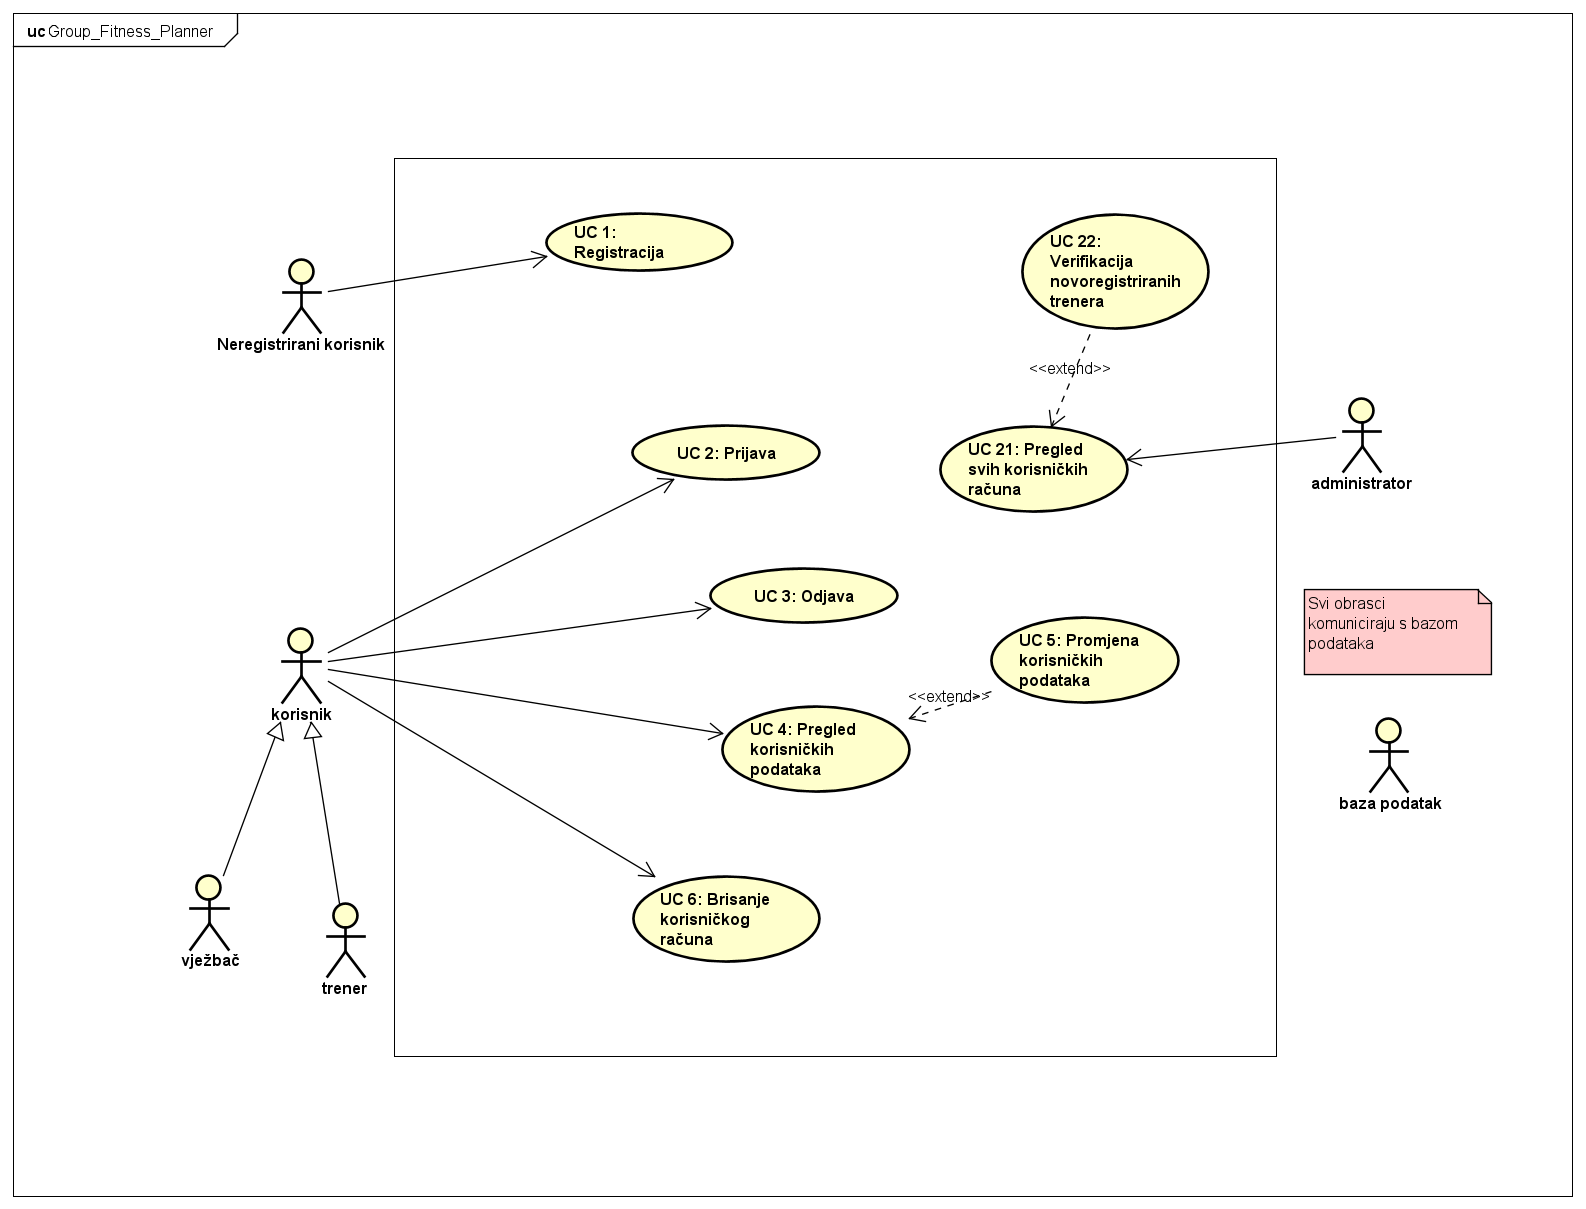
\includegraphics[scale=0.4]{./Dijagrami/UC0_Group_Fitness_Planner.png}
                      \centering
                      \caption{Dijagram obrasca uporabe}
                      \label{fig:promjene}
                \end{figure}
                \begin{figure}[H]
                      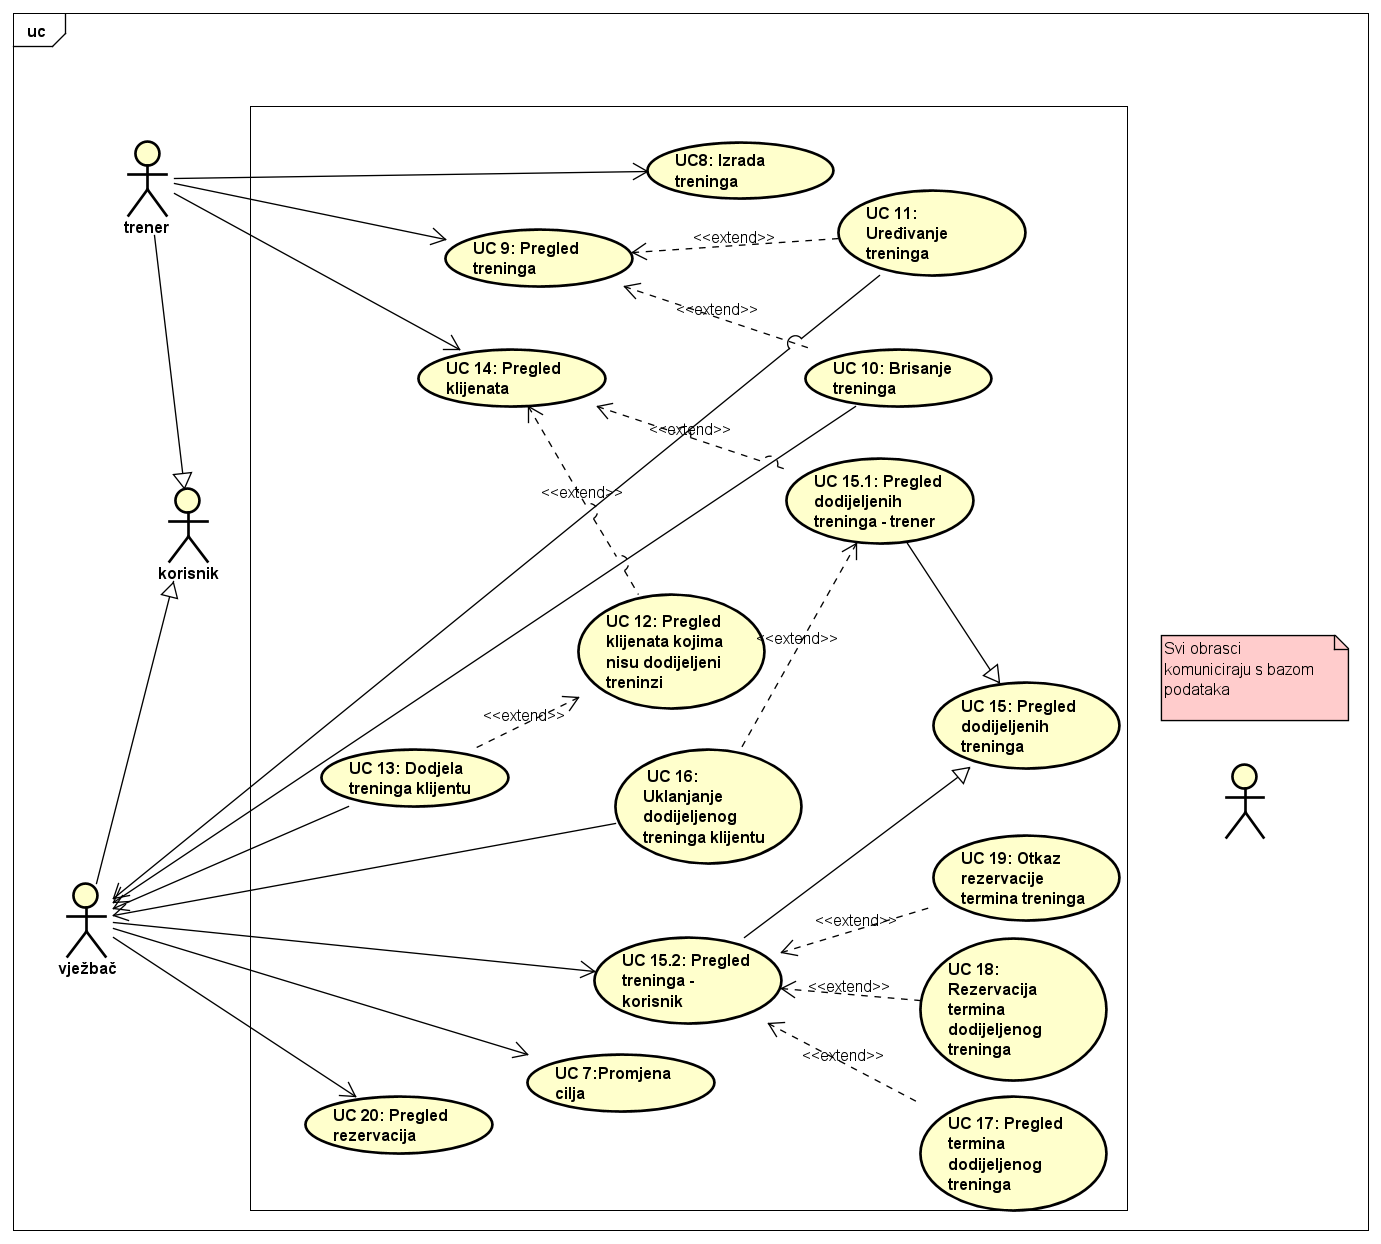
\includegraphics[scale=0.4]{./Dijagrami/UC1_Uloge.png}
                      \centering
                      \caption{Dijagram obrasca uporabe, funkcionalnost vježbača i trenera}
                      \label{fig:promjene}
                \end{figure}
                
				\eject		
				
			\subsection{Sekvencijski dijagrami}
   
	   			\subsubsection{Obrazac uporabe UC1: Registracija}
				\noindent Korisnik bira opciju za registraciju, te poslužitelj prikazuje formu za registraciju. Zatim korisnik unosi svoje ime, prezime, datum rođenja, e-mail adresu i broj telefona. Osmišlja korisničko ime i lozinku za prijavu, te odabire opciju želi li se registrirati kao vježbač ili kao trener. U slučaju da korisnik odabire opciju vježbač, odabire cilj. Po završetku ispunjavanja forme korisnik klikne na gumb registriraj se. Sustav provjerava dostupnost korisničkog imena, e-mail adrese, te ispravnost ostalih unesenih podataka u skladu sa zahtjevima sustava. Ukoliko su podaci ispravni, sustav šalje link za aktivaciju korisničkog računa na upisanu e-mail adresu i obavještava korisnika o uspješnoj registraciji. 

                \begin{figure}[H]
		              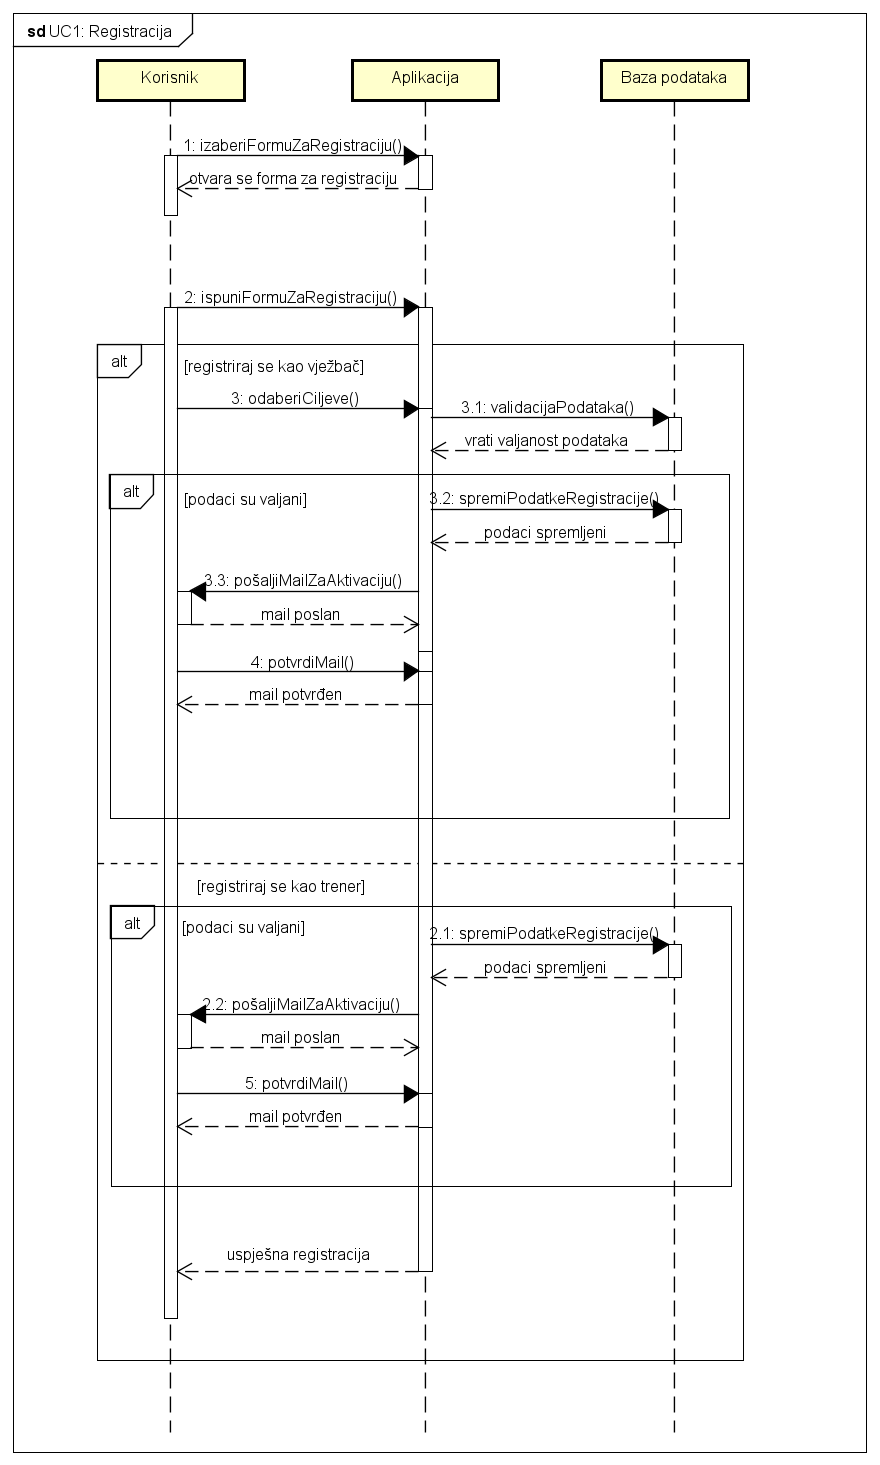
\includegraphics[scale=0.55]{./Dijagrami/UC1_Registracija.png}
		              \centering
		              \caption{Sekvencijski dijagram registracije}
		              \label{fig:promjene}
	            \end{figure}

                \subsubsection{Obrazac uporabe UC8: Izradi trening}
				\noindent Trener bira opciju "Izradi trening". Sustav otvara prozor za izradu treninga s formom za unos podataka o treningu. Trener unosi glavne podatke o treningu i odabire dane u tjednu u kojima bi se izvodio trening. Sustav za svaki dan nudi slobodne termine treninga koje zatim trener odabire za terning u izradi. Na kraju trener odabire opciju "Potvrdi", a sustav provjerava jesu li svi podaci ispravnog oblika. Ukoliko jesu sustav pohranjuje podatke o kreiranom treningu i njegovim terminima te ih sprema u bazu podataka. Ukoliko je sustav utvrdio da je trener unio neispravan oblik podataka o treningu, na zaslonu se pojavi poruka "Došlo je do pogreške".   

                \begin{figure}[H]
		              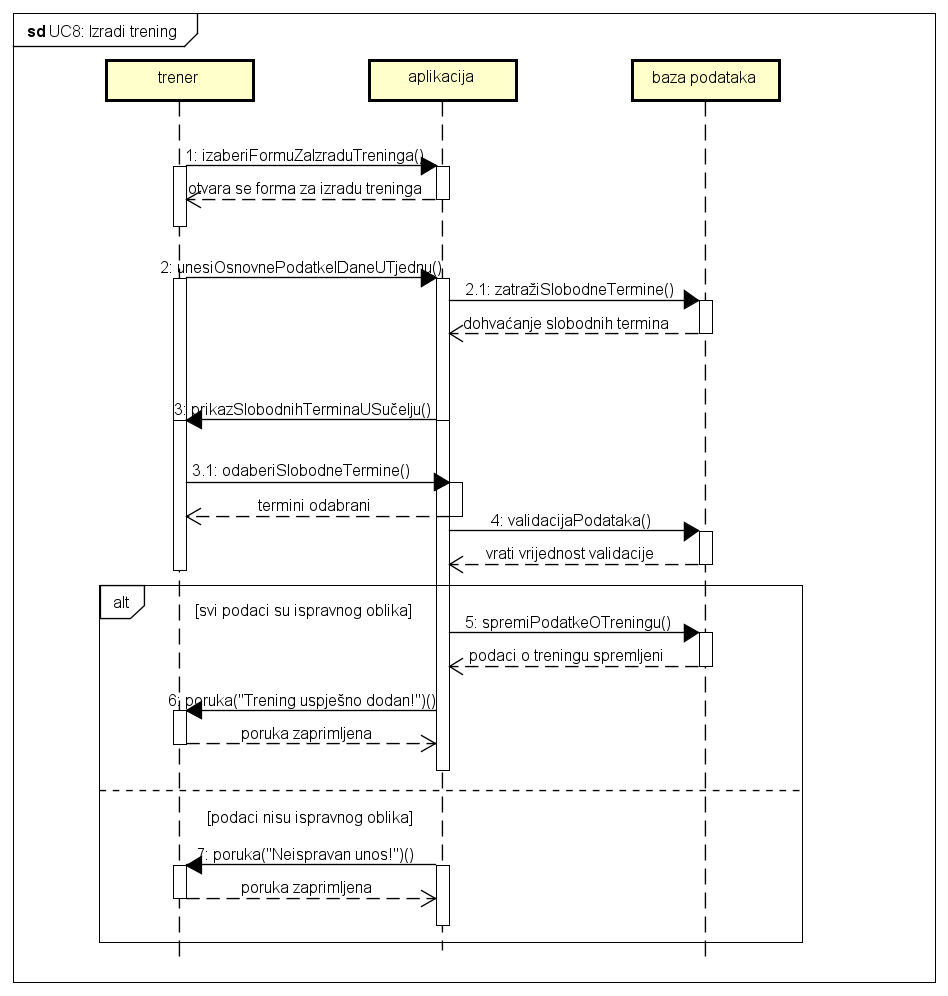
\includegraphics[scale=0.5]{./Dijagrami/UC8_Izradi_trening.png}
		              \centering
		              \caption{Sekvencijski dijagram izrade treninga}
		              \label{fig:promjene}
	            \end{figure}

                \subsubsection{Obrazac uporabe UC10: Dodjeli treninge klijentu}
				\noindent Trener klikom na gumb "Prikaz klijenata bez dodjeljenog treninga" otvara formu. Unutar te forme treneru se prikazuju svi mogući treninzi sa opcijom "Dodijeli". Treneru se odabirom opcije "Dodijeli" omogućuje i unos broja sati predviđenih za odrađivanje odabranih treninga. Trener potvrđuje odabrane treninge klikom na gumb "Spremi". Sustav ispituje ispravnost spremljenih podataka. Ukoliko su podaci ispravni, sustav sperma dodjeljene treninge i broj sati potrebnih da se oni odrade u bazu podataka. Zatim obavještava trenera o uspješno dodjeljenim treninzima iz sučelja aplikacije, a klijenta putem maila. Ukoliko podaci nisu ispravni aplikacija obavještava trenera o neuspješnom unosu treninga. 

                \begin{figure}[H]
		              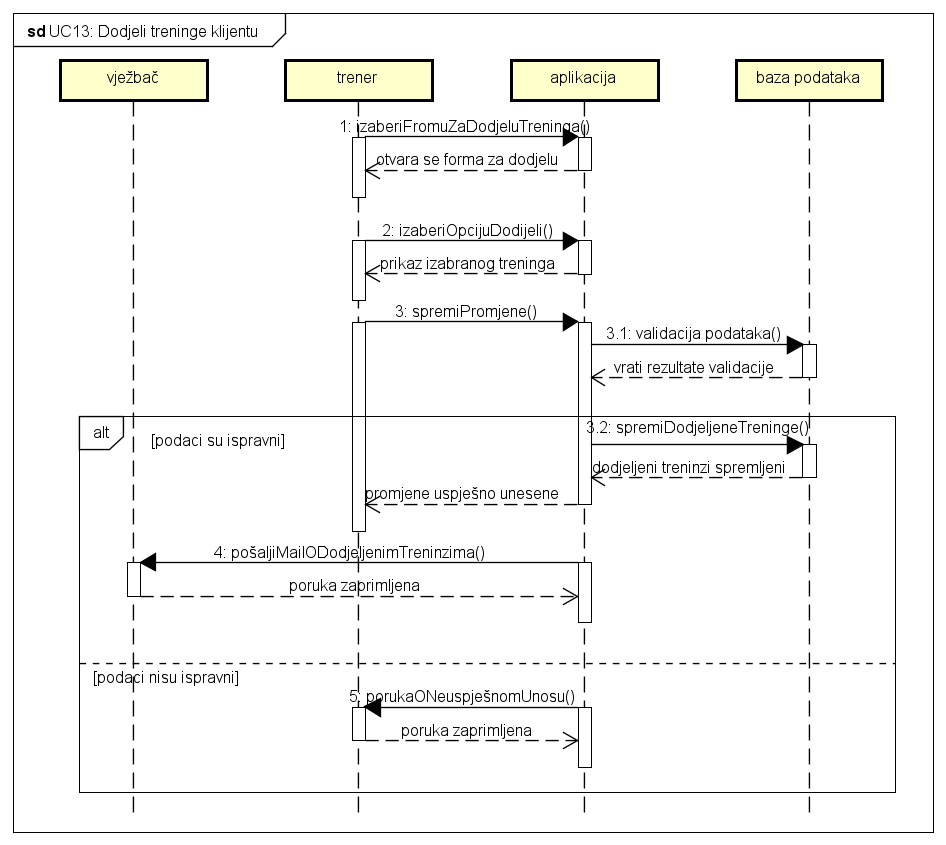
\includegraphics[scale=0.6]{./Dijagrami/UC13_Dodjeli_treninge_klijentu.png}
		              \centering
		              \caption{Sekvencijski dijagram dodjele treninga klijentima}
		              \label{fig:promjene}
	            \end{figure}

             
                \subsubsection{Obrazac uporabe UC12: Rezerviraj termin dodjeljenog treninga}
				\noindent Klijent ima pristup formi "Pregled dodjeljenih treninga". Klijent odabire termin među ponuđenima, a klikom na gumb "Rezerviraj" rezervira termin treninga. Sustav provjerava ograničenja. Ukoliko provjera odobrava rezervaciju treninga, aplikacija unosi podatak o rezervaciji u bazu podataka, smanjuje fond sati klijenta za jedan, smanjuje broj raspoloživim mjesta u rezervaciji treninga, i obavještava klijenta o uspješnoj rezervaciji u sučelju aplikacije. U slučaju neuspješne provjere sustav u sučelju aplikacije izdaje obavijest da rezervaciju nije moguće izvršiti zbog ograničenja.

                \begin{figure}[H]
		              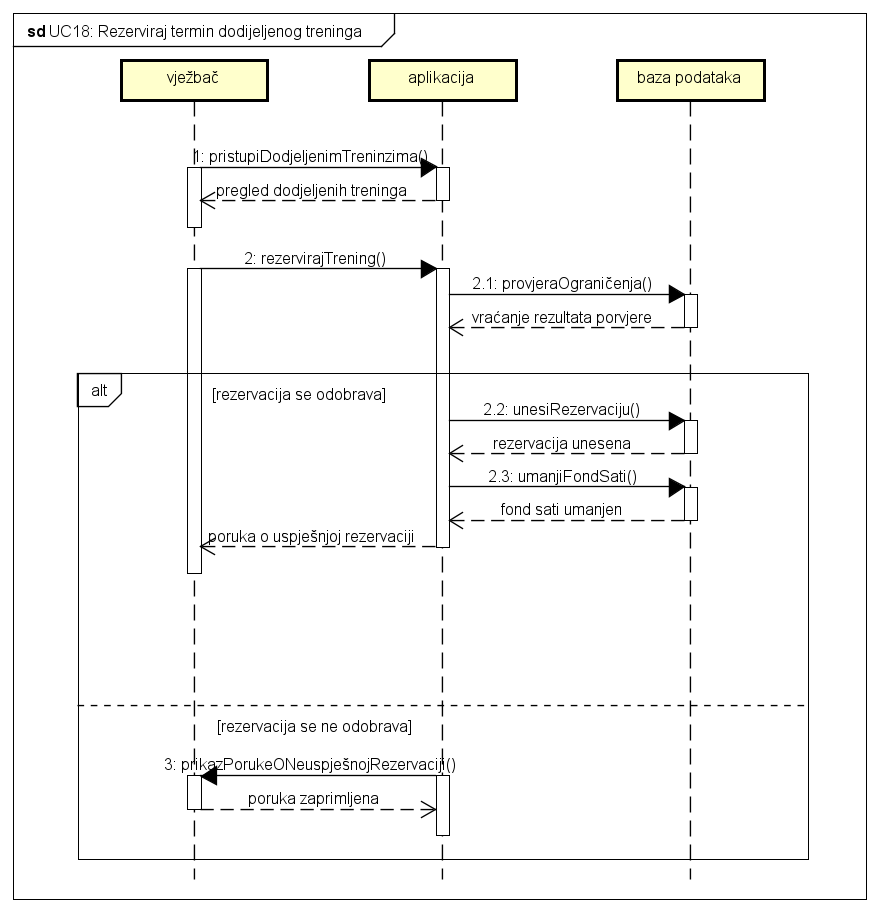
\includegraphics[scale=0.6]{./Dijagrami/UC18_ Rezerviraj_termin_dodijeljenog_treninga.png}
		              \centering
		              \caption{Sekvencijski dijagram rezervacije dodijeljenog termina}
		              \label{fig:promjene}
	            \end{figure}
               \eject
            
	
		\section{Ostali zahtjevi}
		
			%\textbf{\textit{dio 1. revizije}}\\
		 
			 {
			        Aplikacija treba biti izvedena kao web aplikacija kojoj će korisnici pristupati uz pomoć korisničkog imena i lozinke.\newline
                    Aplikacija treba biti jednostavna za korištenje, a sučelje pregledno i intuitivno. Osim toga, aplikacija treba biti prilagođena za rad na različitim uređajima (mobilni uređaj, tablet, PC).\newline
                    Aplikaciju treba implementirati u arhitekturi klijent-poslužitelj. Na poslužiteljskoj strani koristiti programski jezik Java i radni okvir Spring Boot, spremati podatke u relacijsku bazu podataka koristeći JPA, a potrebnu funkcionalnost izložiti kroz REST Web servise. \newline 
                    Na klijentskoj strani implementirati korisničko sučelje u Web pregledniku koristeći React ili Angular, koje se spaja na navedene servise.}
			 
			 
			 
	
	
\chapter{Arhitektura i dizajn sustava}
		
		
	\noindent Komunikacija sa našim sustavom ostvaruje se korištenjem web preglednika koji prikazuje grafičko sučelje naše aplikacije. Korisnička interakcija sa grafičkim sučeljem rezultira slanjem zahtjeva web preglednika prema web poslužitelju na kojem se nalazi naša web aplikacija. \newline
	Iz navedenog možemo definirati \textbf{web preglednik} kao program koji krajnjem korisniku omogućava jednostavno pretraživanje i pregled podataka na Internetu, \textbf{web poslužitelj} kao program koji prima zahtjeve web preglednika, prosljeđuje ih web aplikaciji na obradu te odgovara web pregledniku podacima koji su mu proslijeđeni od strane web aplikacije. \textbf{Web aplikacija} program je koji obrađuje primljene zahtjeve, komunicira s bazom podataka te šalje podatke web poslužitelju za prikaz u web pregledniku.
	\newline 
	U našem slučaju web poslužitelju se pristupa putem REST-a (engl. \textit{Representational State Transfer}) te je odgovor poslužitelja u JSON obliku.
	\newline
	Troslojna arhitektura našeg sustava prezentirana je sljedećim slojevima
	\begin{packed_item}
		\item Sloj interakcije
		\item Sloj servisa
		\item Sloj repozitorija
	\end{packed_item}
	
	
	\noindent Interakcijski sloj predstavlja sučelje aplikacije pomoću kojeg krajnji korisnik iskorištava ostvarene funkcionalnosti aplikacije. 
	\newline 
	Sastoji se od dva podsloja:
	\begin{packed_item}
		\item Prikazni sloj
		\item Kontrolerski sloj 
	\end{packed_item}
	
	\noindent Prikazni sloj dio je \textit{frontend} dijela sustava. Za njegovu implementaciju odabran je React razvojni okvir (engl. \textit{framework}). \newline
	Kontrolerski sloj dio je \textit{backend} dijela sustava. Zadužen je za posluživanje zahtjeva dobivenih od prikaznog sloja.
	\newline\newline
	Servisni sloj naše aplikacije sadržan je unutar \textit{backend} dijela sustava. Sadrži strukture i funkcije čija je zadaća ispunjavanje zamišljenih funkcionalnosti aplikacije. Unutar njega se odrađuju izračuni i obrada podataka koji se onda predaju podatkovnom sloju. \newline\newline
	Repozitorijski je sloj također sadržan unutar već navedenog \textit{backend} dijela sustava. Zadužen je za komunikaciju s bazom podataka i razmjenom navedenih podataka sa servisnim slojem.
	\newline\newline
	Navedeni opis slojeva odgovara MVC arhitekturi (engl. \textit{Model-View-Controller}) čija je osnovna forma prikazana na sljedećoj slici. \newline
	\begin{figure}[H]
		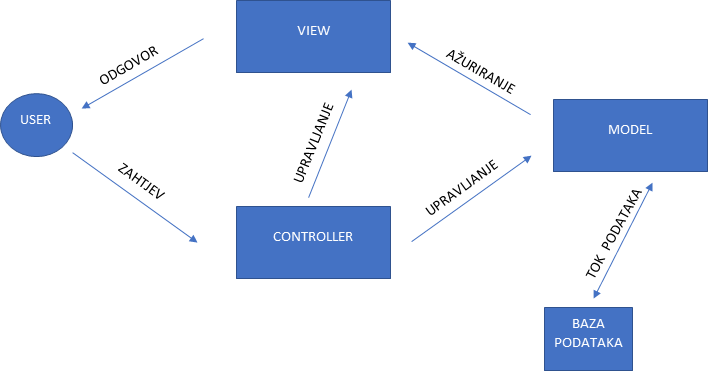
\includegraphics[scale=0.6]{./Slike/mvc-opce.png}
		\centering
		\caption{Opći MVC obrazac}
		\label{fig:promjene}
	\end{figure}
	\noindent Korištenjem Spring razvojnog okvira (engl. \textit{framework}) za razvoj aplikacije sloj prikaza i sloj kontrolera spojeni su unutar jednog sloja (koji možemo zvati sloj interakcije), dok su ostala dva sloja ostala odvojena. 
	\begin{figure}[H]
		
\includegraphics[scale=0.6]{./Slike/mvc-spring.png}
		\centering
		\caption{Spring MVC obrazac}
		\label{fig:promjene}
	\end{figure}
	\noindent Svi navedeni slojevi ostvaruju svoje funkcionalnosti komunikacijom s modelima (engl. models) sustava. Oni su oblikovani na način da apstrahiraju korisnike i elemente sustava te enkapsuliraju atribute potrebne za ostvarenje zamišljenih funkcionalnosti sustava. 
	\newline 
	Spring razvojni okvir (engl. \textit{framework}) pohranjuje strukturu modela unutar baze podataka korištenjem objektno-relacijskog preslikavanja (engl. \textit{object-relational mapping, ORM}) koje pruža alat Hibernate ORM. Preslikavanje se odvija prema predodređenim Java specifikacijama unutar Java Persistence aplikacijskog sučelja (JPA) koje alat kao što je Hibernate ORM implementira. Rezultat je skup tablica unutar odabrane baze podataka koje sadrže atribute modela i atribute veza među modelima.
	\newline
	Sustav upravljanja bazama podataka (engl. \textit{Relation Database Management System, RDBMS}) koji smo odabraili za izradu aplikacije je PostgreSQL. Jednostavno ga je integrirati unutar Spring razvojnog okvira (engl. \textit{framework}) uključivanjem tzv. \textit{dependecya}.
	
			
	\section{Baza podataka}
		
		
	Za potrebe sustava modelirana je relacijska baza podataka koja svojom strukturom modelira stvarni svijet, tj. odnose potrebne aplikaciji. Gradivna jedinka baze je relacija,  tablica definirana svojim imenom i skupom atributa. Zadaća baze podataka brza je i jednostavna pohrana, izmjena i dohvat podataka za daljnju obradu.
	Baza podataka ove aplikacije sastoji se od sljedećih entiteta:
	\begin{packed_item}
		\item User
		\item Client
		\item Coach
		\item Training
		\item Workout
		\item Time
		\item Goals
		\item Schedule
		\item Token
		\item Training\_workouts
		\item Client\_schedules
		\item Coach\_clients
		\item Client\_trainings
	
	\end{packed_item}
	
		\subsection{Opis tablica}
	
	
			\textbf{USER} \newline
	Entitet USER sadržava informacije o korisniku aplikacije. Korisnik može biti trener, klijent i administrator. Sadrži atribute: userID, name, surname, dateOfBirth, username, email, password, contact, role. 
			
			\begin{longtblr}[
				label=none,
				entry=none
				]{
					width = \textwidth,
					colspec={|X[6,l]|X[6, l]|X[20, l]|}, 
					rowhead = 1,
				} %definicija širine tablice, širine stupaca, poravnanje i broja redaka naslova tablice
				\hline \multicolumn{3}{|c|}{\textbf{USER}}	 \\ \hline[3pt]
				\SetCell{LightGreen} userID & BIGINT	&  	jedinstveni identifikator korisnika  	\\ \hline
				name & VARCHAR & ime korisnika		\\ \hline 
				surname & VARCHAR & prezime korisnika	\\ \hline 
				dateOfBirth & DATE & datum rođenja korisnika \\ \hline
				email & VARCHAR & e-mail adresa korisnika \\ \hline 
				username & VARCHAR & korisničko ime korisnika, alternativni ključ  	\\ \hline 
				password & VARCHAR & hash zapis lozinke	\\ \hline 
				contact & VARCHAR & kontakt broj korisnika \\ \hline
				role & ENUM	& uloga korisnika u sustavu	\\ \hline 
			\end{longtblr}
			
			\textbf{CLIENT} \newline
	Entitet CLIENT predstavlja specijalizaciju nad entitetom USER. Sadrži atribute entitete USER te currentGoal, nextGoal, hoursAvailable.
			
			\begin{longtblr}[
				label=none,
				entry=none
				]{
					width = \textwidth,
					colspec={|X[6,l]|X[6, l]|X[20, l]|}, 
					rowhead = 1,
				} %definicija širine tablice, širine stupaca, poravnanje i broja redaka naslova tablice
				\hline \multicolumn{3}{|c|}{\textbf{CLIENT}}	 \\ \hline[3pt]
				\SetCell{LightBlue} currentGoal & VARCHAR & trenutni cilj \\ \hline
				\SetCell{LightBlue} nextGoal & VARCHAR & sljedeći odabrani cilj \\ \hline
			 hoursAvailable & INT & fond sati treninga po mjesecu \\ \hline
			\end{longtblr}
			
			\textbf{COACH} \newline
	Entitet COACH predstavlja specijalizaciju nad entitetom USER. Sadrži atribute eniteta USER i atribut verified koji predstavlja odobrenje administratora
			
			\begin{longtblr}[
				label=none,
				entry=none
				]{
					width = \textwidth,
					colspec={|X[6,l]|X[6, l]|X[20, l]|}, 
					rowhead = 1,
				} %definicija širine tablice, širine stupaca, poravnanje i broja redaka naslova tablice
				\hline \multicolumn{3}{|c|}{\textbf{COACH}}	 \\ \hline[]
				\hline verified & BOOLEAN	&  status verifikacije trenera  	\\ \hline
				
			\end{longtblr}
		
			\textbf{TRAINING} \newline
	Entitet TRAINING sadržava informacije o treningu. Sadrži atribute: trainingID, userID, trainingName, duration, trainingRules. Entitet je u vezi Many-to-Many s entitetom TRAINING\_WORKOUTS preko atributa trainingID.
			
			\begin{longtblr}[
				label=none,
				entry=none
				]{
					width = \textwidth,
					colspec={|X[6,l]|X[6, l]|X[20, l]|}, 
					rowhead = 1,
				} %definicija širine tablice, širine stupaca, poravnanje i broja redaka naslova tablice
				\hline \multicolumn{3}{c}{\textbf{TRAINING}}	 \\ \hline[3pt]
				\SetCell{LightGreen} trainingID & INT	&  	jedinstveni identifikator treninga  	\\ \hline
				\SetCell{LightBlue}coachUserID & INT & jedinstveni identifikator trenera \\ \hline 
				trainingName & VARCHAR & naziv treninga 	\\ \hline 
				duration & TIME & duljina treninga \\ \hline 
				trainingRules & VARCHAR & pravila koja postavlja trener\\ \hline 
			\end{longtblr}
		
			\textbf{WORKOUT} \newline
	Entitet WORKOUT sadržava sve moguće vježbe unutar aplikacije. Sadrži atribute: workoutID, workoutName, workoutTypeID. Entitet je u vezi Many-To-Many s TRAINING\_WORKOUTS preko atributa workoutID, te u vezi Many-To-One s WORKOUT\_TYPE preko atributa workoutTypeID;
		
			\begin{longtblr}[
				label=none,
				entry=none
				]{
					width = \textwidth,
					colspec={|X[6,l]|X[6, l]|X[20, l]|}, 
					rowhead = 1,
				} %definicija širine tablice, širine stupaca, poravnanje i broja redaka naslova tablice
				\hline \multicolumn{3}{|c|}{\textbf{WORKOUT}}	 \\ \hline[3pt]
				\SetCell{LightGreen} workoutID & INT	&  	jedinstveni identifikator vježbe  	\\ \hline
				workoutName & VARCHAR & naziv vježbe 	\\ \hline 
				workoutTypeID & BIGINT & identifikator tipa vježbe \\ \hline 
			\end{longtblr}
		
			\textbf{TIME} \newline
	Entitet TIME sadržava moguće termina treninga unutar dana. Sadrži atribut timeOfday. 
			
			\begin{longtblr}[
				label=none,
				entry=none
				]{
					width = \textwidth,
					colspec={|X[6,l]|X[6, l]|X[20, l]|}, 
					rowhead = 1,
				} %definicija širine tablice, širine stupaca, poravnanje i broja redaka naslova tablice
				\hline \multicolumn{3}{|c|}{\textbf{TIME}}	 \\ \hline[3pt]
				\SetCell{LightGreen} timeOfDay & INT & termin treninga unutar dana  	\\ \hline
			\end{longtblr}	
		
			\textbf{GOALS} \newline
	Entitet GOALS sadržava moguće ciljeve vježbanja za korisnika. Sadrži atribute goalName.
			
			\begin{longtblr}[
				label=none,
				entry=none
				]{
					width = \textwidth,
					colspec={|X[6,l]|X[6, l]|X[20, l]|}, 
					rowhead = 1,
				} %definicija širine tablice, širine stupaca, poravnanje i broja redaka naslova tablice
				\hline 
				\multicolumn{3}{c}{\textbf{GOALS}}	 \\ \hline[3pt]
				\SetCell{LightGreen} goalName & VARCHAR & jedinstveni identifikator i naziv cilja  	\\ \hline
			\end{longtblr}	
			
			\textbf{SCHEDULE} \newline
	Entitet SCHEDULE sadržava informacije o održavanju treninga unutar dana, te broju mjesta slobodnih za određeni trening. Sadrži atribute trainingID, date, timeOfDay, spaceLeft. TrainingID strani je ključ entiteta TRAINING te s atributom date čini primarni ključ.
			
			\begin{longtblr}[
				label=none,
				entry=none
				]{
					width = \textwidth,
					colspec={|X[6,l]|X[6, l]|X[20, l]|}, 
					rowhead = 1,
				} %definicija širine tablice, širine stupaca, poravnanje i broja redaka naslova tablice
				\hline 
				\multicolumn{3}{c}{\textbf{SCHEDULE}}	 \\ \hline[3pt]
				\SetCell{LightGreen} trainingID & BIGINT & jedinstveni identifikator treninga 	\\ \hline
			  \SetCell{LightGreen} date & DATE & datum treninga \\ \hline
			  \ timeOfDay & INT & termin treninga u danu \\ \hline
			  \ spaceLeft & INT & broj slobodnih mjesta \\ \hline
			  \end{longtblr}
			  
	% 		   \textbf{TOKEN} \newline
	% Entitet TOKEN sadržava informacije o novoregistriranom korisniku i generiranom tokenu (string) koji mu je dodijeljen za mail verifikaciju.
		  
	% 		\begin{longtblr}[
	% 			label=none,
	% 			entry=none
	% 			]{
	% 				width = \textwidth,
	% 				colspec={|X[15,l]|X[6, l]|X[20, l]|}, 
	% 				rowhead = 1,
	% 			} %definicija širine tablice, širine stupaca, poravnanje i broja redaka naslova tablice
	% 			\hline 
	% 			\multicolumn{3}{c}{\textbf{TOKEN}}	 \\ \hline[3pt]
	% 			\SetCell{LightGreen} tokenID & BIGINT & jedinstveni identifikator tokena	\\ \hline
	% 		  \SetCell{LightBlue} userID & BIGINT & jedinstveni identifikator korisnika \\ \hline
	% 		  \ token & VARCHAR & token \\ \hline
	% 		  \end{longtblr} 
			  
	\textbf{TRAINING\_WORKOUTS} \newline
	TRAINING\_WORKOUTS predstavlja spojnu tablicu treninga i vježbi koja će se koristiti za određivanje vrste treninga. Sadrži atribute trainingID i workoutID koji su strani ključevi redom tablica TRAINING i WORKOUT.
		  
			\begin{longtblr}[
				label=none,
				entry=none
				]{
					width = \textwidth,
					colspec={|X[15,l]|X[6, l]|X[20, l]|}, 
					rowhead = 1,
				} %definicija širine tablice, širine stupaca, poravnanje i broja redaka naslova tablice
				\hline 
				\multicolumn{3}{c}{\textbf{TRAINING\_WORKOUTS}}	 \\ \hline[3pt]
				\SetCell{LightGreen} trainingID & BIGINT & jedinstveni identifikator treninga 	\\ \hline
			  \SetCell{LightGreen} workoutID & BIGINT & jedinstveni identifikator vježbe \\ \hline
			  \end{longtblr}
			  
			\textbf{CLIENT\_SCHEDULES} \newline
	CLIENT\_SCHEDULES predstavlja spojnu tablicu koja povezuje klijenta s dodijeljenim treninzima i njihovim terminima. Sadrži atribute userID, trainingID, date, reservation. UserID i trainingID redom su strani ključevi iz tablica USER i TRAINING.
		  
			\begin{longtblr}[
				label=none,
				entry=none
				]{
					width = \textwidth,
					colspec={|X[15,l]|X[6, l]|X[20, l]|}, 
					rowhead = 1,
				} %definicija širine tablice, širine stupaca, poravnanje i broja redaka naslova tablice
				\hline 
				\multicolumn{3}{c}{\textbf{CLIENT\_SCHEDULES}}	 \\ \hline[3pt]
				\SetCell{LightGreen} userID & BIGINT & jedinstveni identifikator korisnika 	\\ \hline
			  \SetCell{LightGreen} trainingID & BIGINT & jedinstveni identifikator treninga \\ \hline
			  \SetCell{LightGreen} date & DATE & datum treninga \\ \hline
			  \ reservation & BOOLEAN & potvrda rezervacije termina treninga \\ 
			  \hline
			  \end{longtblr}
		  
			\textbf{COACH\_CLIENTS} \newline
	COACH\_CLIENTS predstavlja spojnu tablicu koja povezuje trenera sa svojim klijentima. Sadrži atribute coachID, clientID. CoachID i ClientID redom su strani ključevi iz tablica COACH i CLIENT u kojima se pojavljuju kao userID.
		  
			 \begin{longtblr}[
				label=none,
				entry=none
				]{
					width = \textwidth,
					colspec={|X[15,l]|X[6, l]|X[20, l]|}, 
					rowhead = 1,
				} %definicija širine tablice, širine stupaca, poravnanje i broja redaka naslova tablice
				\hline 
				\multicolumn{3}{c}{\textbf{COACH\_CLIENTS}}	 \\ \hline[3pt]
				\SetCell{LightGreen} coachID & BIGINT & jedinstveni identifikator trenera 	\\ \hline
			  \SetCell{LightGreen} clientID & BIGINT & jedinstveni identifikator klijenta \\ \hline
			  \end{longtblr}                
			  
			\textbf{CLIENT\_TRAININGS} \newline
	CLIENT\_TRAININGS predstavlja spojnu tablicu koja povezuje klijenta sa dodijeljenim treninzima. Sadrži atribute userID te trainingID. UserID i trainingID redom su strani ključevi iz tablica CLIENT i TRAINING.
		  
			 \begin{longtblr}[
				label=none,
				entry=none
				]{
					width = \textwidth,
					colspec={|X[15,l]|X[6, l]|X[20, l]|}, 
					rowhead = 1,
				} %definicija širine tablice, širine stupaca, poravnanje i broja redaka naslova tablice
				\hline 
				\multicolumn{3}{c}{\textbf{CLIENT\_TRAININGS}}	 \\ \hline[3pt]
				\SetCell{LightGreen} userID & BIGINT & jedinstveni identifikator klijenta  	\\ \hline
			  \SetCell{LightGreen} trainingID & BIGINT & jedinstveni identifikator treninga \\ \hline
			  \end{longtblr}    
			  \textbf{WORKOUT\_TYPE} \newline
	WORKOUT\_TYPE predstavlja tablicu koja sadrži podatke o mogućim tipovima vježbi. Sadrži atribute typeID i workoutType.
		  
			 \begin{longtblr}[
				label=none,
				entry=none
				]{
					width = \textwidth,
					colspec={|X[15,l]|X[6, l]|X[20, l]|}, 
					rowhead = 1,
				} %definicija širine tablice, širine stupaca, poravnanje i broja redaka naslova tablice
				\hline 
				\multicolumn{3}{c}{\textbf{WORKOUT\_TYPE}}	 \\ \hline[3pt]
				\SetCell{LightGreen} typeID & BIGINT & jedinstveni identifikator tipa vježbe  	\\ \hline
			  \ workoutType & VARCHAR & naziv tipa vježbe \\ \hline
			  \end{longtblr}               
		  
		  
		  
		  
		  
		\subsection{Dijagram baze podataka}
			\begin{figure}[H]
		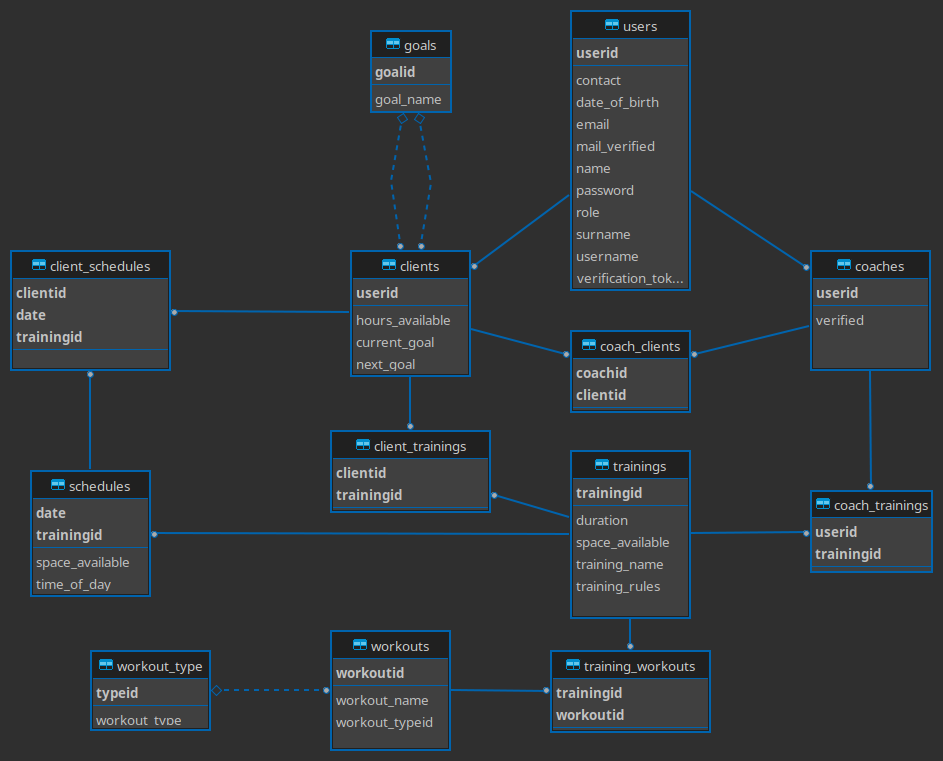
\includegraphics[scale=0.45]{./Dijagrami/relations.png}
		\centering
		\caption{Dijagram tablica unutar baze podataka}
		\label{fig:promjene}
	\end{figure}
		
		\eject
		
		
	\section{Dijagram razreda}
		\noindent Dijagrami razreda pokazuju povezanost komponenti sustava te daju jasniji uvid u arhitekturu i dizajn aplikacije. Podijeljeni su u 4 podkategorije (sa dodatnim prikazom metoda servisa) :
		 \begin{packed_item}    
			\item Modeli - Slika 4.4
			\item Kontroleri u vezi sa servisima - Slika 4.5
			\item Servisi u vezi sa repozitorijima - Slika 4.6                
			\item Repozitoriji - Slika 4.7
                \item Servisi - Slika 4.8
		
		\end{packed_item}
		\noindent U modelima je važno istaknuti postojanje glavne klase za korisnike zvane "User". Iz nje su izvedene klase klijenta (vježbač) i trenera sa potrebnim atributima specijalizacije.
		\begin{figure}[H]
		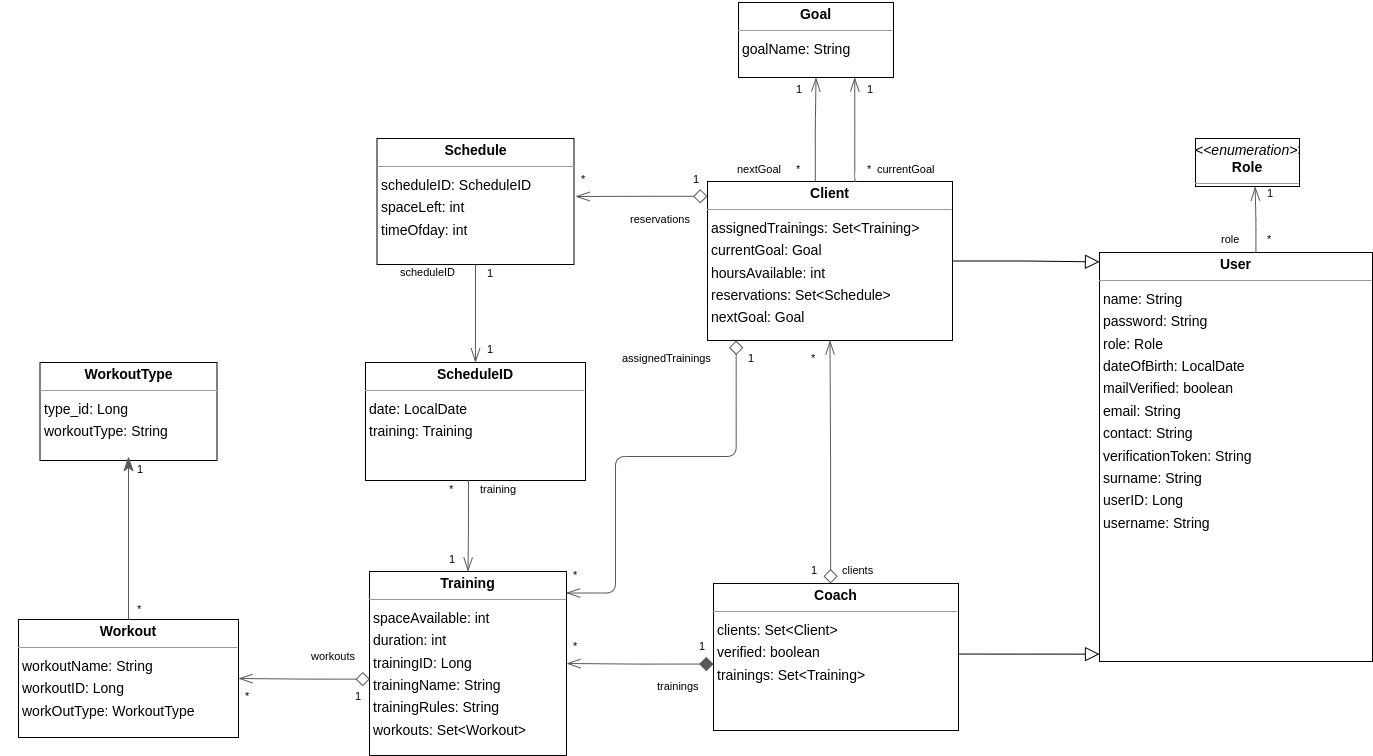
\includegraphics[scale=0.425]{./Dijagrami/domain.png}
		\centering
		\caption{Modeli}
		\label{fig:promjene}
	\end{figure}
    \noindent Servisi ostvaruju funkcionalnosti sustava komunikacijom sa bazom podataka preko repozitorija. Prikazani su neki glavni servisi (i njihove implementacije) koji su zaduženi za opće korisnike (tj. funkcionalnosti koje imaju i klijenti i treneri) te pojedinačni servisi za svaku od navedenih uloga.
	\begin{figure}[H]
		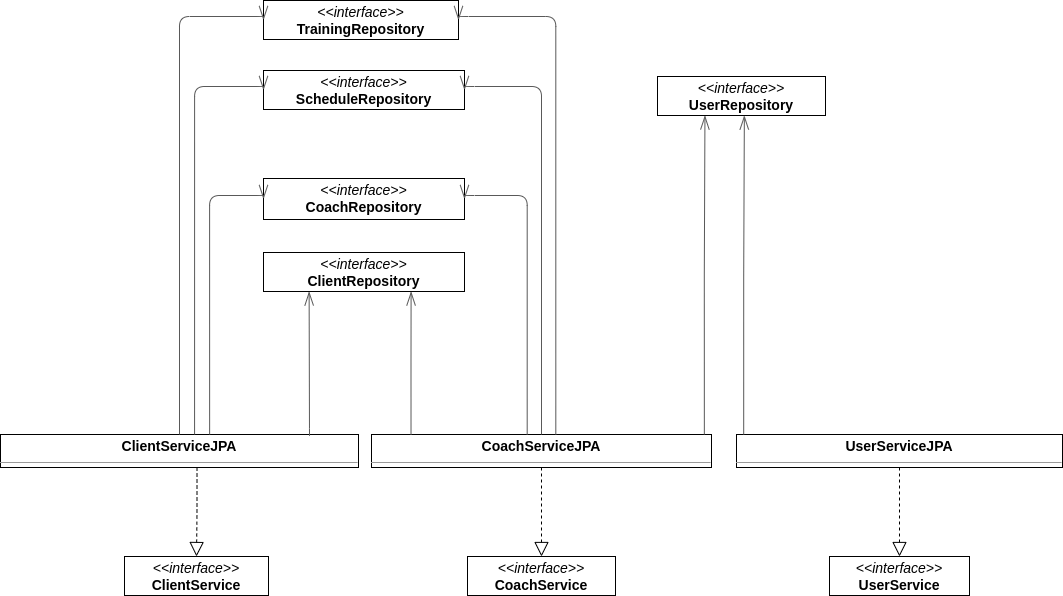
\includegraphics[scale=0.425]{./Dijagrami/services_repositories.png}
		\centering
		\caption{Servisi u vezi sa repozitorijima}
		\label{fig:promjene}
	\end{figure}
	\noindent Kontroleri i servisi čine najvažniji dio sustava jer sadržavaju logiku potrebnu za ostvarivanje zamišljenih funkcionalnosti. Dobivanjem zahtjeva sa \textit{frontend} strane sustava, kontroleri prosljeđuju iste odgovarajućim servisima (sa kojima su u vezi). Ovdje su prikazani najvažniji servisi (i odgovarajuće implementacije) i kontroleri za ostvarivanje funkcionalnosti trenera, klijenata i korisnika kao zajedničkog naziva istih.
	\begin{figure}[H]
		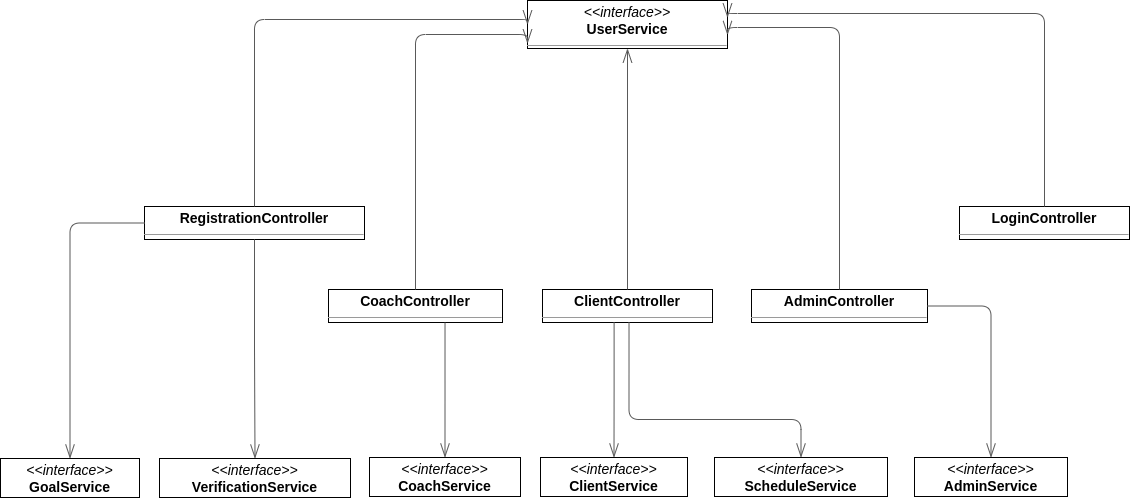
\includegraphics[scale=0.4]{./Dijagrami/controllers_services.png}
		\centering
		\caption{Kontroleri u vezi sa servisima}
		\label{fig:promjene}
	\end{figure}
	\noindent Repozitoriji nasljeđuju osnovni repozitorij unutar Spring Boot radnog okvira (JpaRepository). Navedeni omogućuje nekoliko standardnih operacija nad odgovajućim entitetima (spremanje, brisanje, dohvaćanje...). Ostale funkcionalnosti se ostvaruju komunikaciju sa bazom podataka koristeći prilagođenih query upita (čija je funkcionalnost vidljiva u nazivu na prikazanoj slici).
	\begin{figure}[H]
		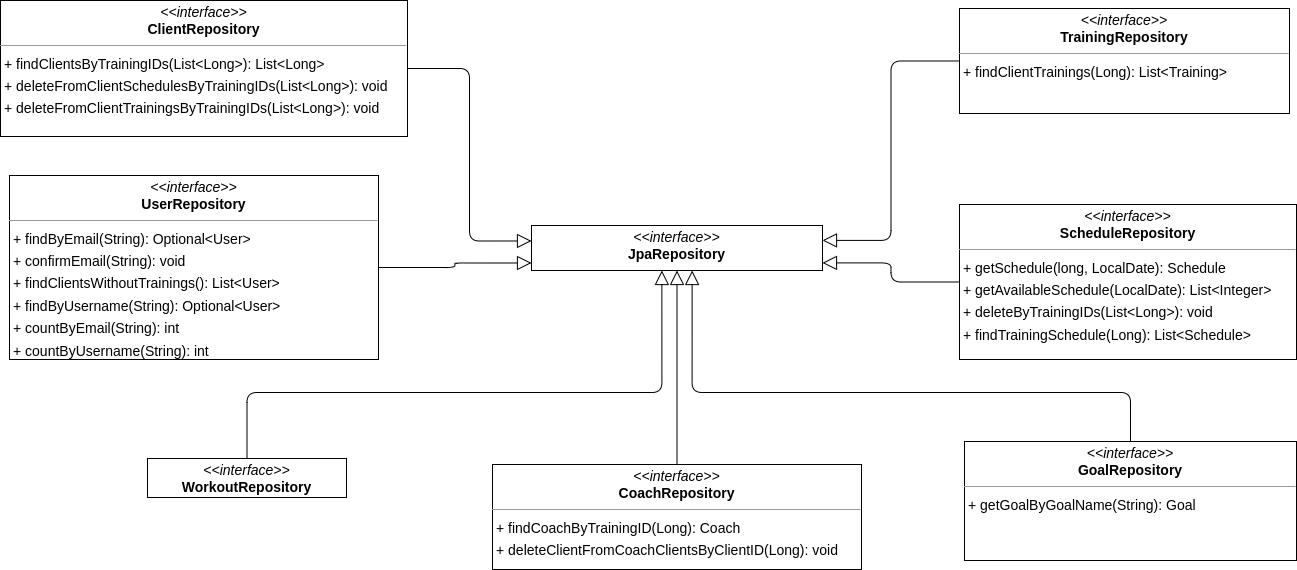
\includegraphics[scale=0.35]{./Dijagrami/repository.png}
		\centering
		\caption{Repozitoriji}
		\label{fig:promjene}
	\end{figure}
        \noindent Radi izbjegavanja zbijenosti na dijagramu servisa i repozitorija izdvojili smo razrede servisa i prikazali njihove implementirane funkcije na sljedećem dijagramu.
	\begin{figure}[H]
		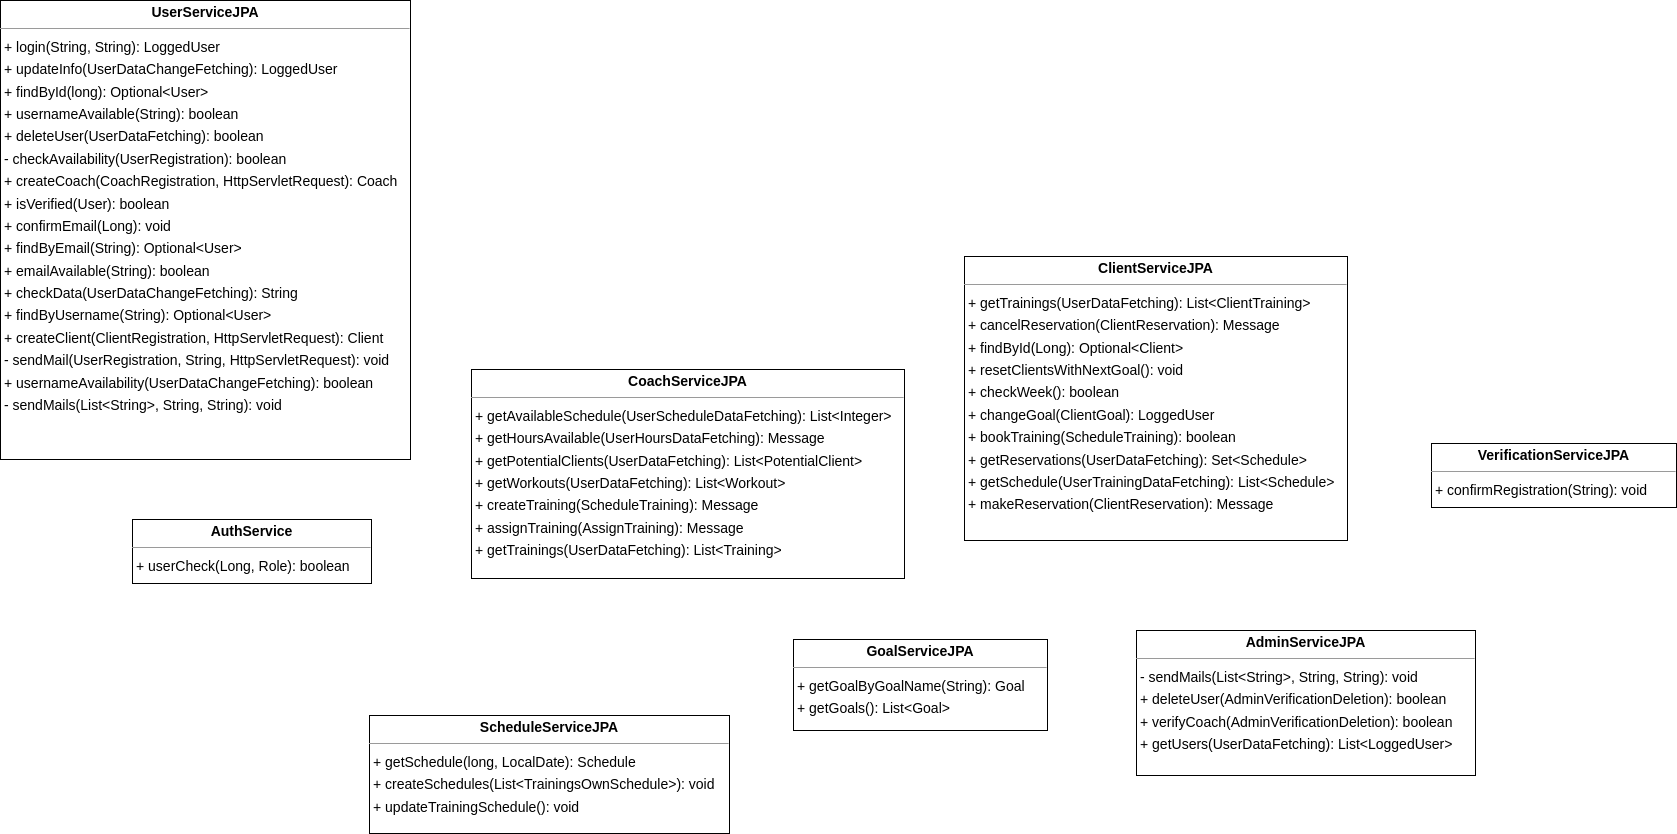
\includegraphics[scale=0.275]{./Dijagrami/services_methods.png}
		\centering
		\caption{Implementirane funkcije servisa}
		\label{fig:promjene}
	\end{figure}
	
		
		%\textbf{\textit{dio 2. revizije}}\\			
		
		%\textit{Prilikom druge predaje projekta dijagram razreda i opisi moraju odgovarati stvarnom stanju implementacije}
		
		
		
		%\eject
	
	%\section{Dijagram stanja}
		
		
	\noindent Dijagram stanja prikazuje stanja objekata te prijelaze među stanjima ovisno o događajima. Slika 4.9 prikazuje dijagram stanja za registriranog korisnika, točnije, vježbača. Prijavom u sustav otvara se početna stranica "Moj profil" na kojoj se mogu pregledati osobni podatci i obrisati račun. Početna stranica je, uz pregled treninga, pregled rezervacija i odjavu, vidljiva i dostupna iz svakog stanja. Na stranici pregleda treninga prikazani su svi treninzi dodijeljeni klijentu te postoji mogućnost odabira jednog od njih. Time se dobiva uvid u sve termine odabranog treninga koji se mogu rezervirati. Na stranici "Pregled rezervacija" prikazani su svi trenutno rezervirani termini logiranog vježbača koji se mogu i otkazati. Na stranici promjene korisničkih podataka dostupna je forma u koju se upisuju podatci za promjenu. 
  
	\begin{figure}[H]
		 \centering
		 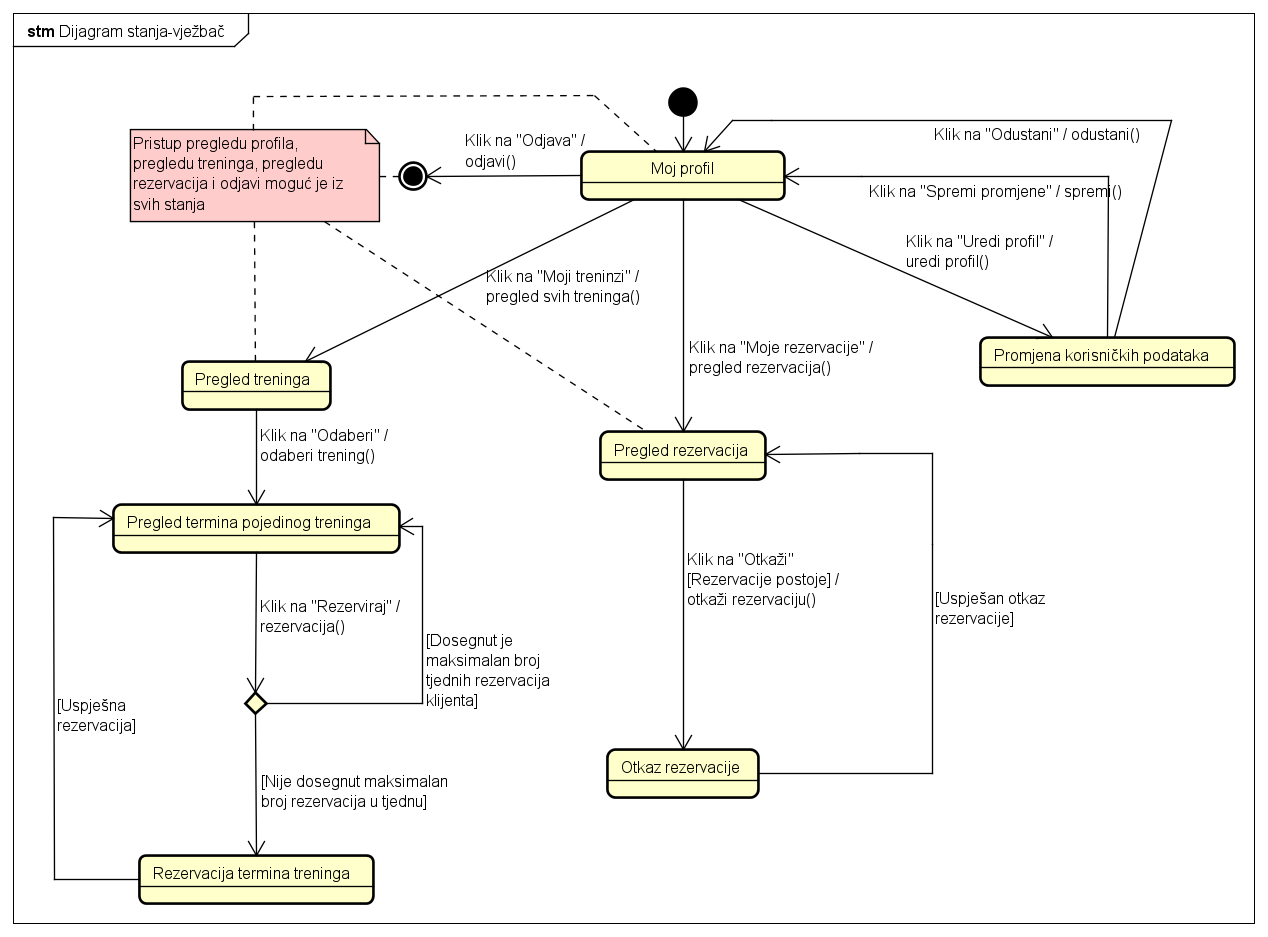
\includegraphics[width=\linewidth]{./Dijagrami/dijagramStanja-vjezbac.png}
		 \caption{Dijagram stanja}
		 \label{fig:Dijagram stanja}
	\end{figure}
		
		%\eject 
	
	%\section{Dijagram aktivnosti}
		
		%\textbf{\textit{dio 2. revizije}}\\
		
		 %\textit{Potrebno je priložiti dijagram aktivnosti s pripadajućim opisom. Dijagram aktivnosti treba prikazivati značajan dio sustava.}
        \noindent \newline Dijagram aktivnosti je ponašajni UML dijagram koji modelira ponašanje nizom akcija, a služi za detaljan prikaz upravljačkog i podatkovnog toga pojedinog segmenta aplikacije (najčešće pojedinih obrazaca uporabe). Dijagramom aktivnosti pogodno je opisivati sinkronizaciju i konkurentnost značajki. 
        \newline Uz našu aplikaciju implementirali smo dijagram aktivnost za obrazac uporabe 5:  „Promjeni korisničke podatke“ kako bismo prikazali podatkovni tok uređivanja postojećih korisničkih profila. 

        \begin{figure}[H]
		      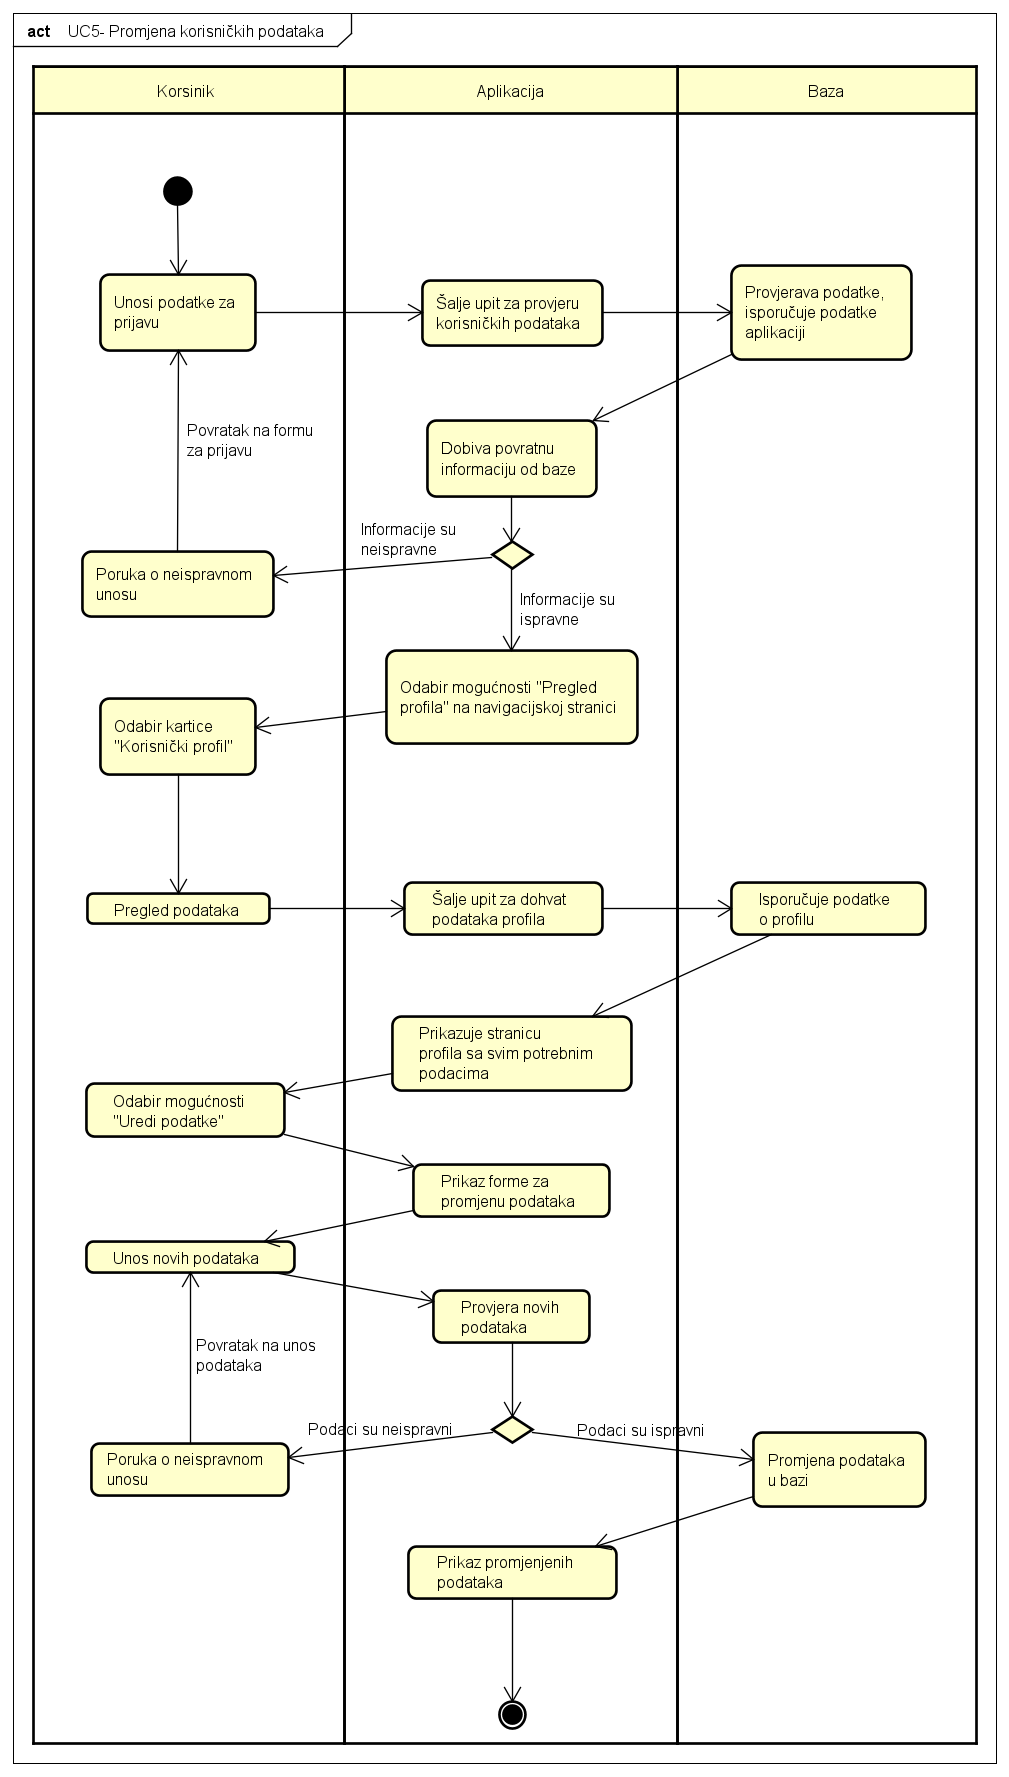
\includegraphics[scale=0.45]{./Dijagrami/UC5_Promjena_korisničkih_podataka_activity.png}
		      \centering
		      \caption{Dijagram aktivnosti za obrazac uporabe 5: "Promjena korisničkih podataka"}
		      \label{fig:promjene}
	   \end{figure}

		
		%\eject
	%\section{Dijagram komponenti}
	
		%\textbf{\textit{dio 2. revizije}}\\
	
		 %\textit{Potrebno je priložiti dijagram komponenti s pripadajućim opisom. Dijagram komponenti treba prikazivati strukturu cijele aplikacije.}

        \noindent \newline Dijagram komponenti je strukturni, statički UML dijagram koji vizualizira organizaciju i međuovisnost interne strukture implementacijskih komponenata, te odnos programske potpore prema okolini. Koristan je za stjecanje okvirne ideje o implementaciji sustava, bez ulaženja u prevelike detalje. 
        \newline Naša aplikacija podijeljena je u četiri glavne komponente: web preglednik (ciljana platforma za pogon aplikacije) koji dohvaća odgovarajuću frontend i backend logiku poštujući internetske komunikacijske protokole, frontend koji dohvaća odgovarajuće HTML, CSS i .js datoteke koje sadrže kod korisničkog sučelja, backend zadužen da dohvat i obradu podataka iz korisničkog sučelja i baze podataka i posreduje komunikaciji navedenih komponenti, te samu SQL bazu podataka.\newline Komponenti frontend logike pristupa se preko sučelja za dohvat HTML-a, CSS-s i .js datoteka iz web preglednika. Centralni dio frontenda je router datoteka (u našem slučaju App.js) zadužena za usklađivanje rada i dohvaćanje željenih komponenti koje su niže u hijerarhiji frontend logike. Svaka komponenta unutar frontend komponente na grafu sadržava ugnježđene komponente u čiju strukturu radi razumljivosti grafa ne ulazimo, a to označava da svaka komponenta ovisi o React libraryju. \newline Komponenta backend logike sa web preglednikom povezana je preko sučelja REST (zathjevi GET, POST, DELETE). Zahtjevi se nakon primitka prvo prosljeđuju kontrolerima, subkomponentama backenda zaduženim za prihvat i isporuku servisima. Servisi su subkomponente backenda koji pomoću svojih sučelja komuniciraju sa kontrolerima i prihvaćaju podatke koji se u njima nalaze, te ih pomoću JPA sučelja prosljeđuju repozitorijima. Repozitoriji omogućuju komunikaciju između servisa i baze podataka. Povezani su sučeljem s SQL bazom podataka. Prijenos podataka između komponenti backend logike ostvaren je „Data transfer object“ klasama pa sve komponente backenda imaju ovisnost prema njima. Svaka komponenta unutar backend komponente na grafu sadržava ugnježđene komponente u čiju strukturu radi razumljivosti grafa ne ulazimo, a to označava da svaka komponenta ovisi o Spring libraryju. 

        \begin{figure}[H]
		    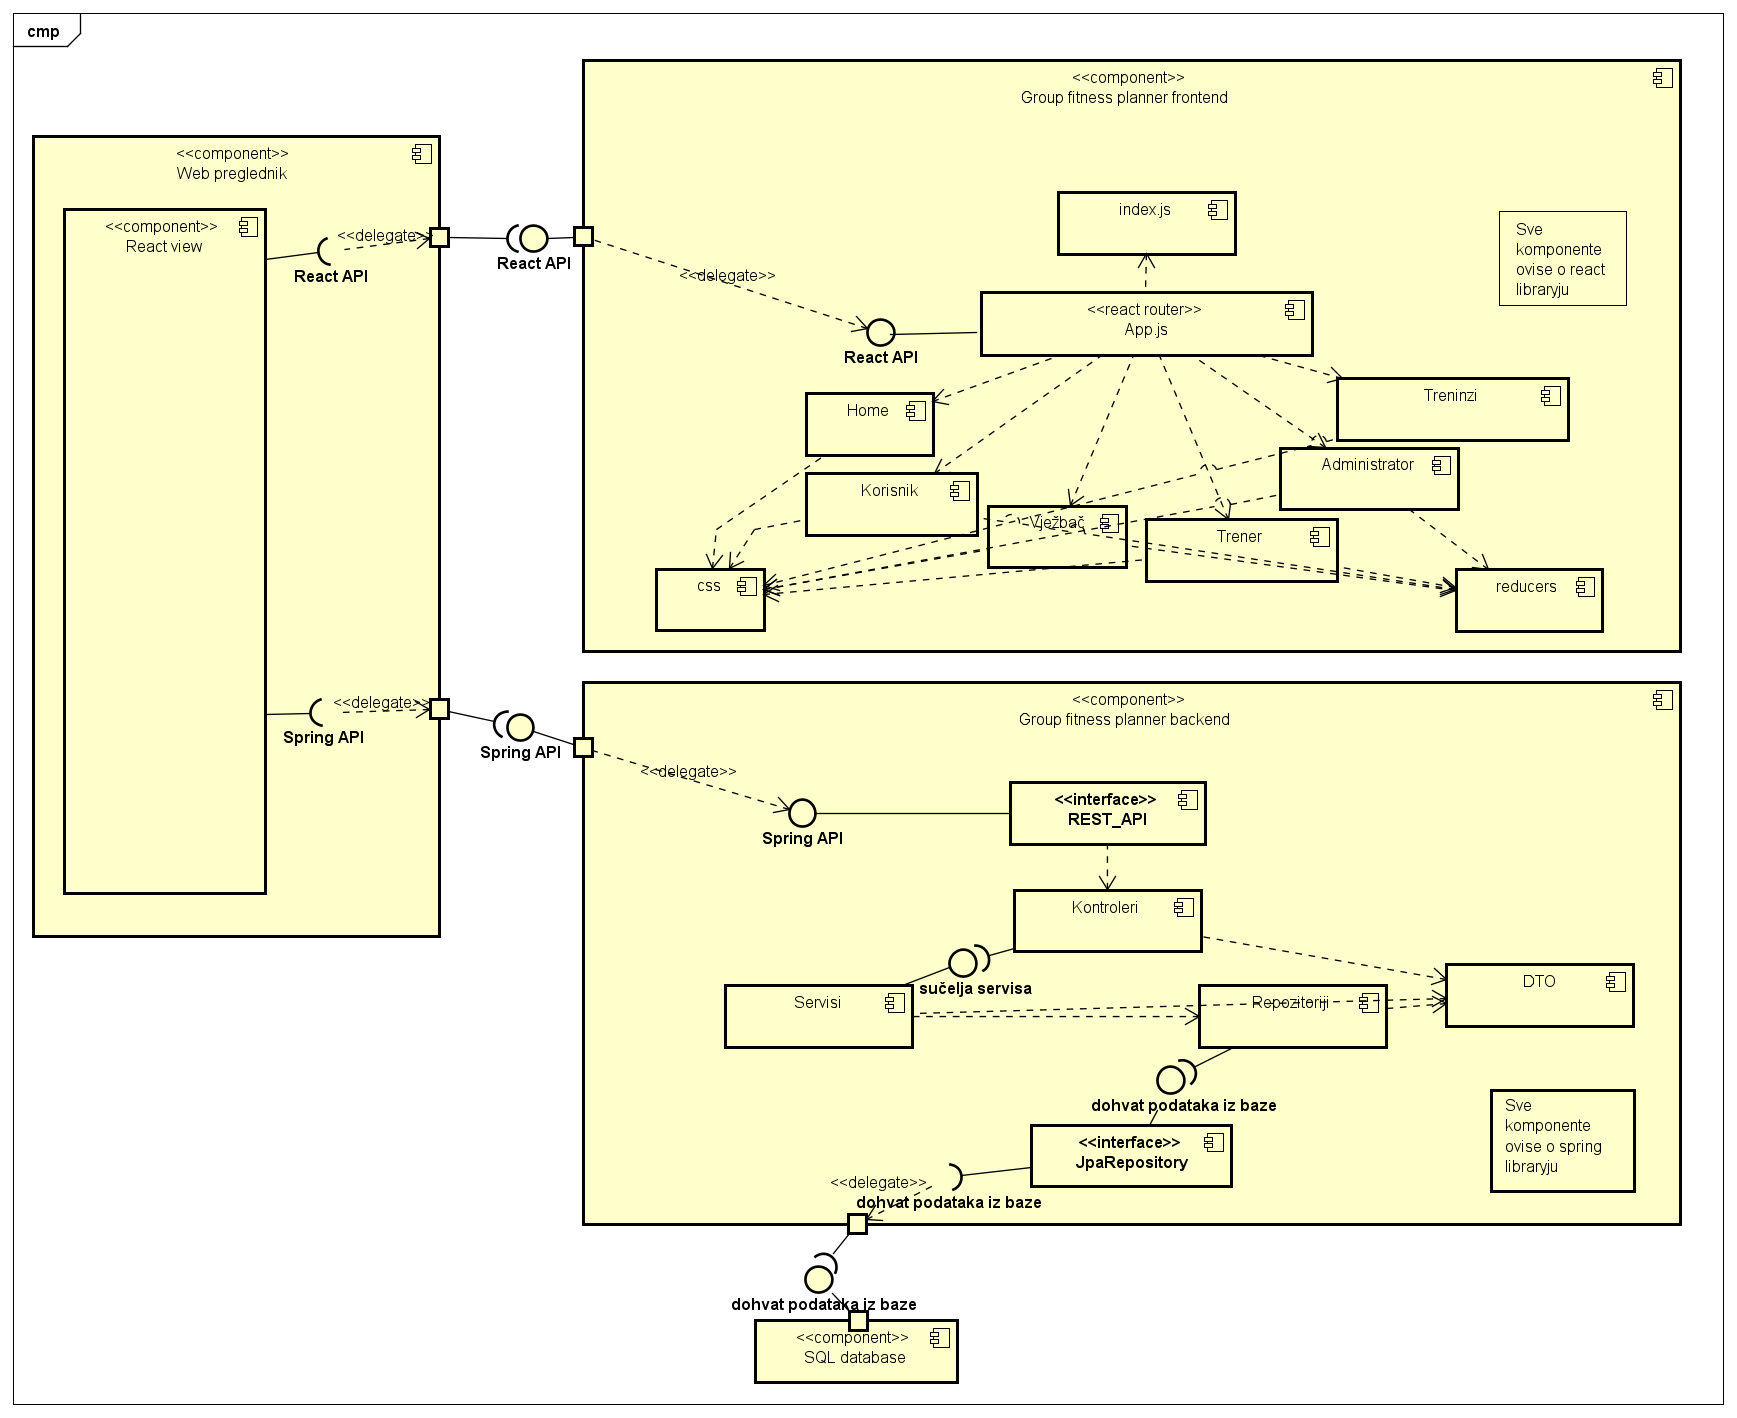
\includegraphics [scale=0.35]{./Dijagrami/Dijagram_komponenti.png}
		      \centering
		      \caption{Dijagram komponenti aplikacije}
		      \label{fig:promjene}
	   \end{figure}

	%\chapter{Implementacija i korisničko sučelje}
		
		
		\section{Korištene tehnologije i alati}
		
			% \textbf{\textit{dio 2. revizije}}
			
			%  \textit{Detaljno navesti sve tehnologije i alate koji su primijenjeni pri izradi dokumentacije i aplikacije. Ukratko ih opisati, te navesti njihovo značenje i mjesto primjene. Za svaki navedeni alat i tehnologiju je potrebno \textbf{navesti internet poveznicu} gdje se mogu preuzeti ili više saznati o njima}.
			
			\subsection{Frontend tehnologije}
            U izradi korisničkog sučelja, točnije \textit{frontend} dijela aplikacije korišten je popularni razvojni okvir \href{https://reactjs.org}{React}. Korištenjem programskog jezika JavaScript React omogućava jednostavnu izradu interaktivnih sučelja temeljenu na React komponentama. Komponente je moguće strukturirati za ponovno korištenje i dijeljenje kroz cijeli projekt (a i druge projekte) što olakšava samu izradu i održavanje. Za uređivanje koda je korišten \href{https://code.visualstudio.com}{Visual Studio Code}.
            \subsection{Backend tehnologije}
			 
		Programski jezik \textit{backend} dijela aplikacije je \href{https://www.java.com/en/download/help/whatis_java.html}{Java}. Korišten je razvojni okvir \href{https://spring.io/projects/spring-boot}{Spring Boot} za čiji je \textit{management} upotrijebljen alat \href{https://maven.apache.org}{Maven}. Tijekom razvoja aplikacije korišten je \href{https://www.h2database.com}{H2} (in-memory) sustav za upravljanje bazama podataka, dok je za \textit{deployanu} verziju korišten sustav \href{https://www.postgresql.org}{PostgreSQL}. Razvojna okruženja korištena na \textit{backendu} su \href{https://www.jetbrains.com/idea/}{InteliJ IDEA} i \href{https://www.eclipse.org}{EclipseIDE}.

            \subsection{Deployment}
            Aplikacija je puštena u pogon na oblaku (engl. cloud) \href{https://render.com}{Render}. Render omogućava povezivanje sa servisom \href{https://gitlab.com}{GitLab} te olakšava puštanje proizvoda u pogon.

            \subsection{Dokumentacija} 
            Za dokumentaciju programskog rješenja korišten je online latex editor. Za crtanje UML dijagrama korišten je Astah i IntelliJ IDEA IDE.

            \subsection{Timska komunikacija} 
            Za timsku komunikaciju korišteni su alati Whatsapp, Discord i Microsoft Teams. 
            
		\section{Ispitivanje programskog rješenja}
			
			%\textbf{\textit{dio 2. revizije}}\\
			 % \textit{U ovom poglavlju je potrebno opisati provedbu ispitivanja implementiranih funkcionalnosti na razini komponenti i na razini cijelog sustava s prikazom odabranih ispitnih slučajeva. Studenti trebaju ispitati temeljnu funkcionalnost i rubne uvjete.}
			\subsection{Ispitivanje komponenti}
			% \textit{Potrebno je provesti ispitivanje jedinica (engl. unit testing) nad razredima koji implementiraju temeljne funkcionalnosti. Razraditi \textbf{minimalno 6 ispitnih slučajeva} u kojima će se ispitati redovni slučajevi, rubni uvjeti te izazivanje pogreške (engl. exception throwing). Poželjno je stvoriti i ispitni slučaj koji koristi funkcionalnosti koje nisu implementirane. Potrebno je priložiti izvorni kôd svih ispitnih slučajeva te prikaz rezultata izvođenja ispita u razvojnom okruženju (prolaz/pad ispita). }
             \noindent \textbf{ 1. ispitni slučaj - pokušaj dodjele rezervacije za trening koji ne postoji}
            \newline U ovom testu ispituje se mogućnost dodjele nepostojeće rezervacije, točnije rezervacije termina treninga koji ne postoji u bazi podataka. Očekuje se iznimka (engl. exception) na servisnom sloju klijenta te ispis poruke u skladu s navedenom iznimkom.
            \begin{figure}[H]
		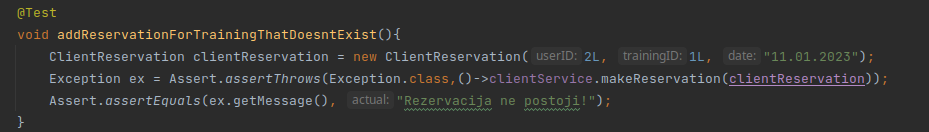
\includegraphics[scale=0.575]{./Slike/test1.png}
		\centering
		\caption{1. test}
		\label{fig:promjene}
	    \end{figure}
            \noindent \textbf{ 2. ispitni slučaj - pokušaj dodjele rezervacije za trening koji nije dodijeljen klijentu}
            \newline U ovom testu ispituje se mogućnost dodjele rezervacije treninga koji nije u treninzima koji su dodijeljeni određenom klijentu, točnije onih koje mu je dodijelio trener. Očekuje se iznimka na servisnom sloju klijenta te ispis poruke u skladu s navedenom iznimkom.
            
            \begin{figure}[H]
		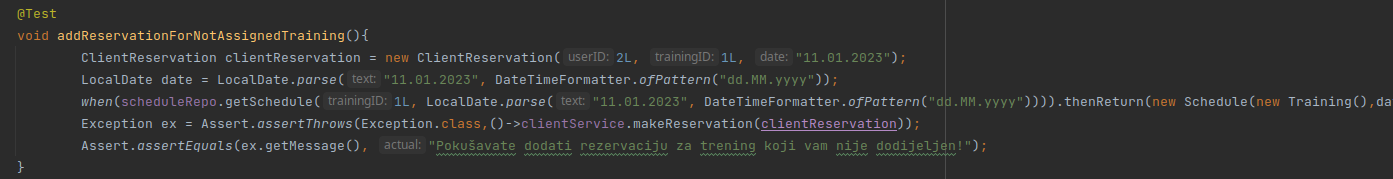
\includegraphics[scale=0.4]{./Slike/test2.png}
		\centering
		\caption{2. test }
		\label{fig:promjene}
	    \end{figure}
            \noindent \textbf{ 3. ispitni slučaj - pokušaj izrade treninga bez prethodne verifikacije od admina}
            \newline U ovom testu ispituje se mogućnost izrade treninga bez prethodne verifikacije trenera od administratora aplikacije. Očekuje se iznimka na servisnom sloju trenera prilikom provjere verfikacije te ispis poruke u skladu s navedenom iznimkom.
            
            \begin{figure}[H]
		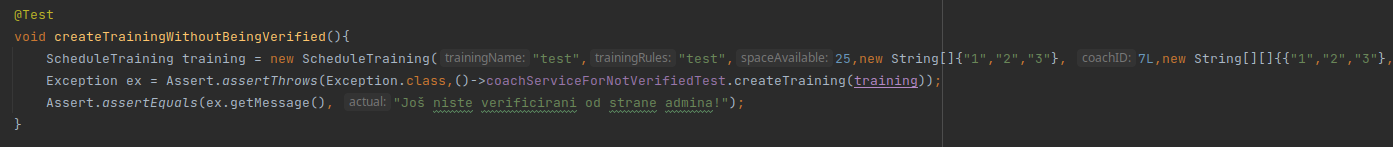
\includegraphics[scale=0.375]{./Slike/test3.png}
		\centering
		\caption{3. test }
		\label{fig:promjene}
	    \end{figure}
            \noindent \textbf{ 4. ispitni slučaj - pokušaj izrade treninga sa prethodnom verifikacijom od admina}
            \newline U ovom testu ispituje se mogućnost izrade treninga nakon verifikacije trenera od administratora aplikacije. Očekuje se uspješna izrada treninga i povratna informacija o istome.
            
            \begin{figure}[H]
		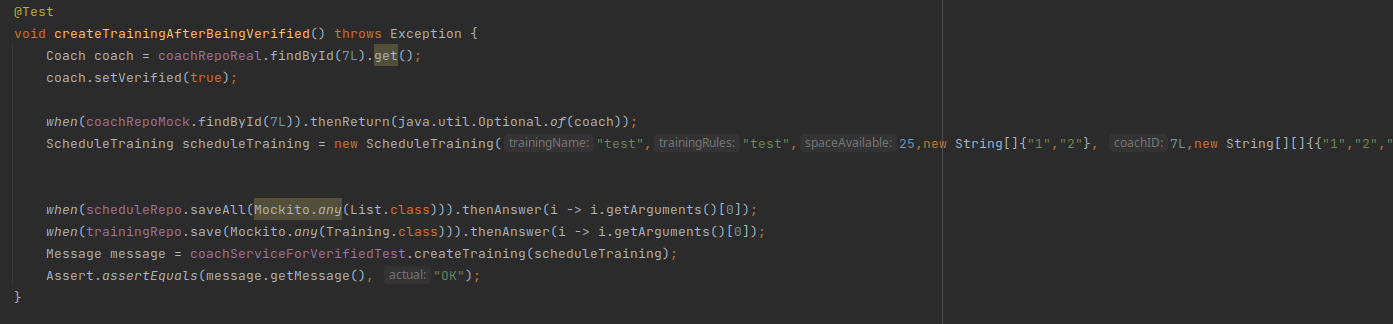
\includegraphics[scale=0.375]{./Slike/test4.png}
		\centering
		\caption{4. test }
		\label{fig:promjene}
	    \end{figure}
            \noindent \textbf{ 5. ispitni slučaj - pokušaja prijave pogrešnom lozinkom}
            \newline U ovom testu ispituje se mogućnost prijave klijenta u aplikaciju pogrešnom lozinkom. Pretpostavka je da je klijent prethodno instanciran i spremljen u bazu podataka s korisničkim imenom kao na slici, a lozinkom password123 te je odgovor servisnog sloja zaduženog za provjeru podataka iznimka s prikladnom porukom o istoj.
     
            \begin{figure}[H]
		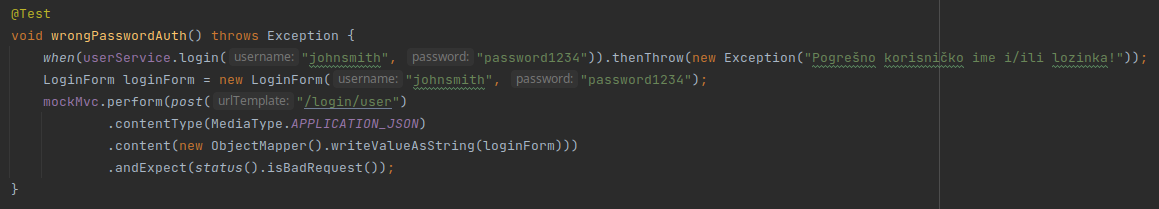
\includegraphics[scale=0.45]{./Slike/test5.png}
		\centering
		\caption{5. test }
		\label{fig:promjene}
	    \end{figure}

            \noindent \textbf{ 6. ispitni slučaj - pokušaj promjene cilja u nepostojeći}
            U ovom testu ispituje se mogućnost promjene cilja klijenta u cilj koji nije definiran unutar baze podataka. Sustav neće dozvoliti takvu promjenu te će se dogoditi iznimka s prikladnom porukom o istoj.
     
            \begin{figure}[H]
		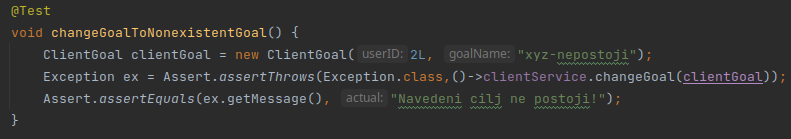
\includegraphics[scale=0.65]{./Slike/test6.png}
		\centering
		\caption{6. test }
		\label{fig:promjene}
	    \end{figure}
     
            \noindent \textbf{Prikaz rezultata testova}
            \newline Testovi komponenti su uspješno provedeni što je vidljivo na priloženoj slici.
            \begin{figure}[H]
		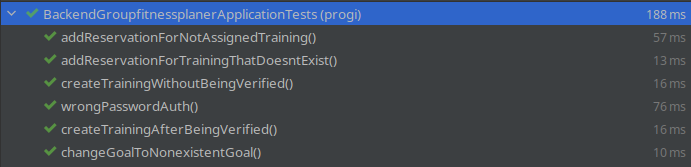
\includegraphics[scale=0.65]{./Slike/test_results.png}
		\centering
		\caption{Rezultati testova }
		\label{fig:promjene}
	    \end{figure}
			
			
			
			\subsection{Ispitivanje sustava}
			
			%  \textit{Potrebno je provesti i opisati ispitivanje sustava koristeći radni okvir Selenium\footnote{\url{https://www.seleniumhq.org/}}. Razraditi \textbf{minimalno 4 ispitna slučaja} u kojima će se ispitati redovni slučajevi, rubni uvjeti te poziv funkcionalnosti koja nije implementirana/izaziva pogrešku kako bi se vidjelo na koji način sustav reagira kada nešto nije u potpunosti ostvareno. Ispitni slučaj se treba sastojati od ulaza (npr. korisničko ime i lozinka), očekivanog izlaza ili rezultata, koraka ispitivanja i dobivenog izlaza ili rezultata.\\ }
			 
			%  \textit{Izradu ispitnih slučajeva pomoću radnog okvira Selenium moguće je provesti pomoću jednog od sljedeća dva alata:}
			%  \begin{itemize}
			%  	\item \textit{dodatak za preglednik \textbf{Selenium IDE} - snimanje korisnikovih akcija radi automatskog ponavljanja ispita	}
			%  	\item \textit{\textbf{Selenium WebDriver} - podrška za pisanje ispita u jezicima Java, C\#, PHP koristeći posebno programsko sučelje.}
			%  \end{itemize}
		 % 	\textit{Detalji o korištenju alata Selenium bit će prikazani na posebnom predavanju tijekom semestra.}
			
			% \eject 

            \noindent \textbf{1. ispitni slučaj sustava: Verifikacija trenera (administrator)}
            \newline \textbf{Postupak}:
            \begin{enumerate}
                
            \item Otvaranje početne stranice

            \item Odabir veze "Pregled korisnika"

            \item Odabir gumba "Potvrdi trenera"

            \item Odabir gumba "OK" u obavještajnom prozoru

            \end{enumerate}
            \textbf{Očekivani rezultati:}
            
		\begin{enumerate}
		    \item Prikaz početne stranice
                \item Prikaz stranice za pregled korisnika
                \item Prikaz obavještajnog prozora s porukom "Jeste li sigurni da želite potvrditi trenera?"
                \item Zatvaranje obavještajnog prozora i uklanjanje gumba "Potvrdi trenera"
		\end{enumerate}
            \begin{figure}[H]
		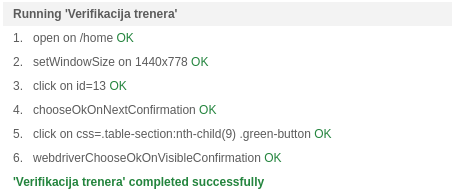
\includegraphics[scale=1]{./Slike/verifikacija_trenera.png}
		\centering
		\caption{1. Selenium test}
		\label{fig:promjene}
	    \end{figure}
     \noindent \textbf{2. ispitni slučaj sustava: Verifikacija trenera (administrator)}
            \newline \textbf{Postupak}:
            \begin{enumerate}
                
            \item Otvaranje početne stranice

            \item Odabir veze "Stvori treninga"

            \item Unos podataka o treningu i terminima treninga

            \item Odabir gumba "Stvori trening"

            \item Odabir gumba "OK" u obavještajnom prozoru

            \end{enumerate}
            \textbf{Očekivani rezultati:}
            
		\begin{enumerate}
		    \item Prikaz početne stranice
                \item Prikaz stranice za izradu treninga
                \item Prikaz obavještajnog prozora s porukom "Uspješno stvoren trening" (nakon 4.)
                \item Zatvaranje obavještajnog prozora
		\end{enumerate}
            \begin{figure}[H]
		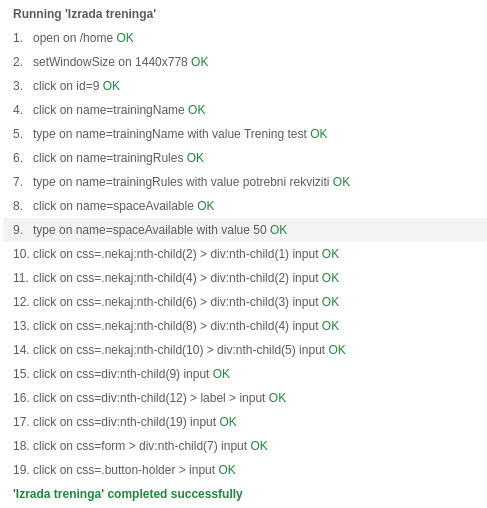
\includegraphics[scale=1]{./Slike/izrada_treninga.png}
		\centering
		\caption{2. Selenium test}
		\label{fig:promjene}
	    \end{figure}
     \noindent \textbf{3. ispitni slučaj sustava: Dodjela treninga klijentu (trener)}
            \newline \textbf{Postupak}:
            \begin{enumerate}
                
            \item Otvaranje početne stranice

            \item Odabir veze "Moji klijenti"

            \item Odabir gumba "Dodijeli trening"

            \item Odabir gumba "Odaberi trening" (moguć višestruki odabir)

            \item Unos fonda sati klijenta

            \item Odabir gumba "Potvrdi odabir"

            \item Odabir gumba "OK" u obavještajnom prozoru

            \end{enumerate}
            \textbf{Očekivani rezultati:}
            
		\begin{enumerate}
		    \item Prikaz početne stranice
                \item Prikaz stranice za pregled klijenata bez treninga
                \item Prikaz stranice za pregled mogućih treninga za dodjelu
                \item Prikaz obavještajnog prozora s porukama "OK" (nakon 6.)
                \item Zatvaranje obavještajnog prozora
		\end{enumerate}
            \begin{figure}[H]
		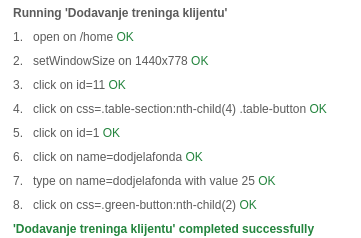
\includegraphics[scale=1]{./Slike/dodjela_treninga_klijentu.png}
		\centering
		\caption{3. Selenium test}
		\label{fig:promjene}
	    \end{figure}
     
     \noindent \textbf{4. ispitni slučaj sustava: Rezervacija termina treninga (klijent)}
            \newline \textbf{Postupak}:
            \begin{enumerate}
                
            \item Otvaranje početne stranice

            \item Odabir veze "Moji treninzi"

            \item Odabir gumba "Odaberi"
            
            \item Odabir gumba "Rezerviraj"

            \item Odabir gumba "OK" u obavještajnom prozoru

            \end{enumerate}
            \textbf{Očekivani rezultati:}
            
		\begin{enumerate}
		    \item Prikaz početne stranice
                \item Prikaz stranice za pregled treninga
                \item Prikaz stranice za pregled termina treninga
                \item Prikaz obavještajnog prozora s porukom "Uspješno ste rezervirali trening!"
                \item Zatvaranje obavještajnog prozora i zatamnjivanje gumba "Rezerviraj"
		\end{enumerate}
            \begin{figure}[H]
		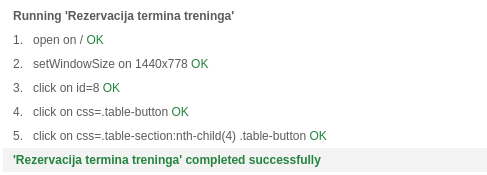
\includegraphics[scale=1]{./Slike/rezervacija_termina_treninga.png}
		\centering
		\caption{4. Selenium test}
		\label{fig:promjene}
	    \end{figure}
		
		\section{Dijagram razmještaja}
			
			% \textbf{\textit{dio 2. revizije}}
			
			 % \textit{Potrebno je umetnuti \textbf{specifikacijski} dijagram razmještaja i opisati ga. Moguće je umjesto specifikacijskog dijagrama razmještaja umetnuti dijagram razmještaja instanci, pod uvjetom da taj dijagram bolje opisuje neki važniji dio sustava.}
                Specifikacijski dijagram razmještaja prikazuje raspodjelu komponenata sustava po lokacijama te odnos sklopovlja i programa. Uočavamo komunikaciju između računala klijenta putem web preglednika i udaljenog poslužitelja (koji sadrži web aplikaciju sa svojim \textit{backend} i \textit{frontend} elementima te poslužitelja baze podataka). Navedena arhitektura sustava naziva se \textit{klijent-poslužitelj} te je u njenoj izvedbi za komunikaciju između dviju navedenih strana korišten protokol HTTP.
			\begin{figure}[H]
		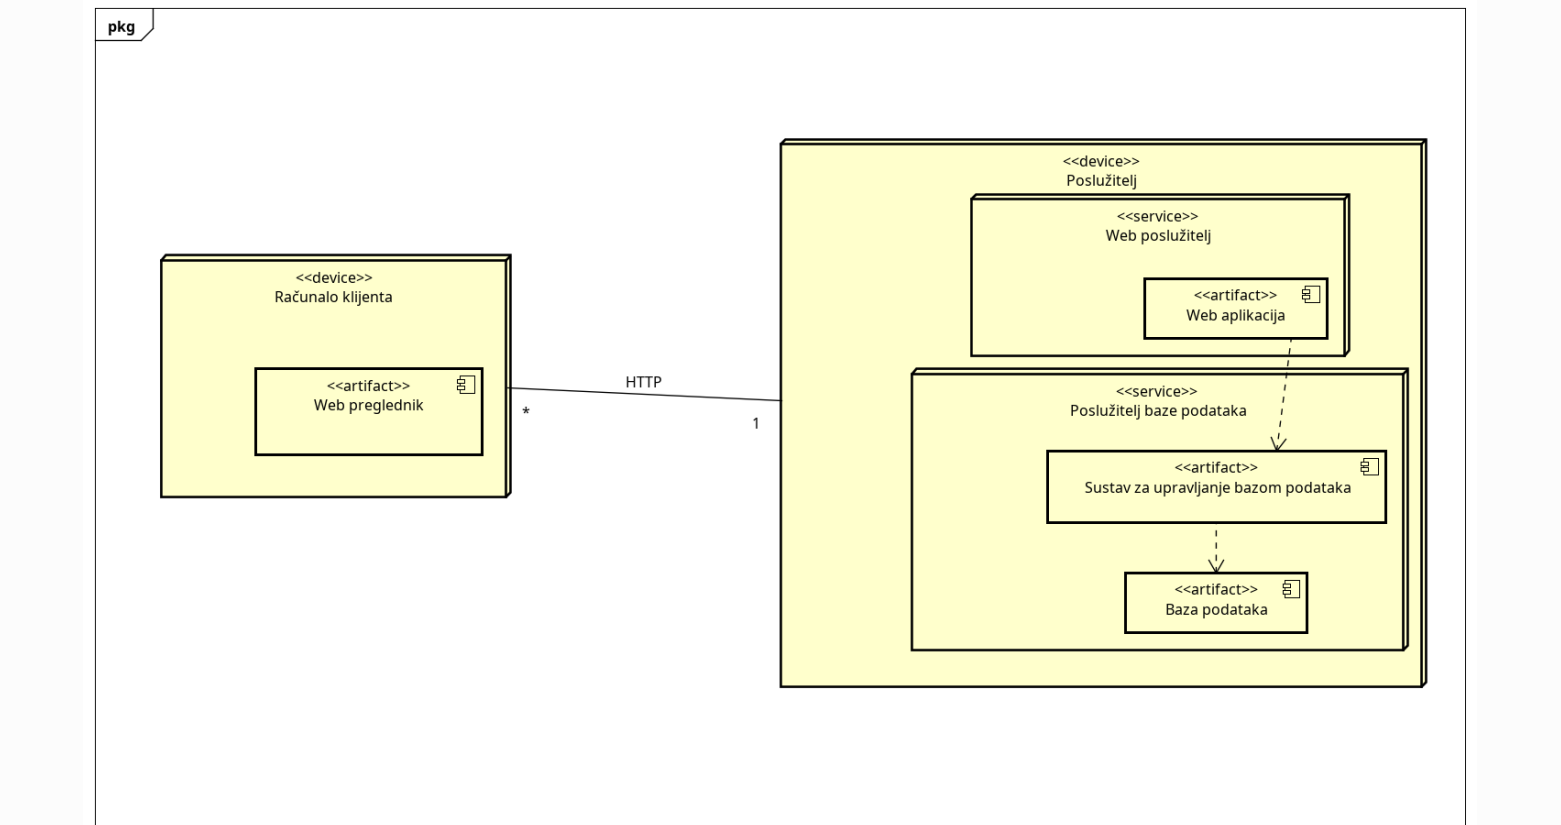
\includegraphics[scale=0.3]{./Dijagrami/dijagram_razmjestaja.png}
		\centering
		\caption{Specifikacijski dijagram razmještaja}
		\label{fig:promjene}
	\end{figure}
			\eject 
		
		
		
		\section{Upute za puštanje u pogon}
            \subsection{Upute za puštanje u pogon na javnom poslužitelju}

            {Aplikacija je puštena u pogon na javnom poslužitelju „Render“. On pruža mogućnost posluživanja web servisa, kao i PostgreSQL baze podataka.\\
            Puštanje u pogon sadržava korake:
            \item \textbf{- kreiranje baze podataka}
            \item \textbf{- puštanje backenda u pogon na javnom poslužitelju}
            \item \textbf{- puštanje frontenda u pogon na javom poslužitelju\\}

            {Bazu podataka kreirali smo i njome upravljamo diretkno iz servisa Render, jer on omogućuje tu opciju. Baza sadržava podatke potrebne za njeno povezivanje sa web servisima. }
            \begin{figure}[H]
                      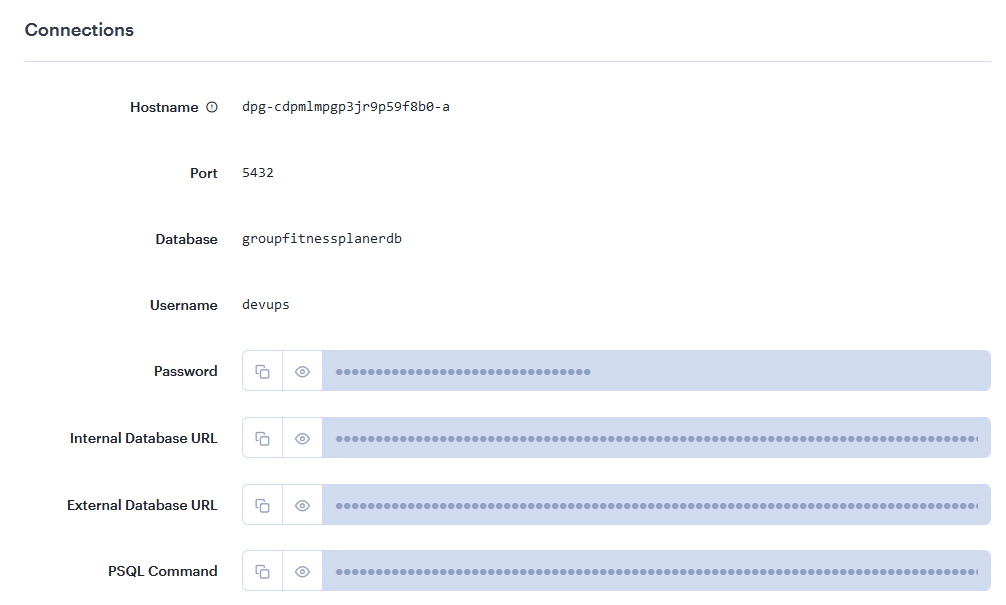
\includegraphics[scale=0.5]{./Slike/baza.png}
                      \centering
                      \caption{Render sučelje za upravljanje bazom podataka}
                      \label{fig:promjene}
                \end{figure}

            {Kako bismo uspješno prenjeli backend aplikacije na web poslužitelj, bilo je potrebno dodati Dockerfile koji upravlja i posreduje komunikaciji backenda i Mavena, alata pomoću kojeg Java projekti postaju sinkronizirani sa Apache HTTP serverima. Također, bilo je potrebno povezati kreiranu bazu podataka sa backendom. Konfiguracija environment varijabli u application.properties datoteci svojstava nužno je da bismo mogli postavili adresu, korisničko ime i lozinku baze podataka na produkciji. Također, opcija kreiranja web servisa u Renderu zahtjeva dodavanje potrebnih varijabli okruženja koje treba kopirati iz danih connections-a baze podataka, postavljanje putanje za Dockerfile. }
            \begin{figure}[H]
                      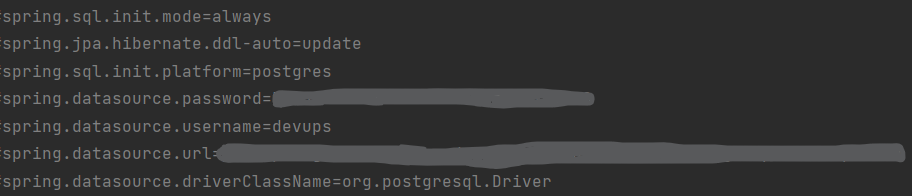
\includegraphics[scale=0.5]{./Slike/config.png}
                      \centering
                      \caption{Konfiguracija postavki za povezivanje backenda sa bazom podataka}
                      \label{fig:promjene}
                \end{figure}

            {Kako bismo uspješno prenjeli frontend, bilo je potrebno u package.json dodati zavisnosti potrebne za puštanje u pogon, primarno proxy-middleware, dotnev, express. Također, bilo je potrebno dodati setupProxy.js koji služi kao server za lokalno razvijanje, app.js u kojem se nalazi express server za produkcijski proxy, kao i izmjeniti package.json dodavanjem "start-prod": "node app.js" skripte, koja navigira front da komunicira preko app.js filea. Opcija kreiranja web servisa u Renderu zahtjevala je postavljanje build komande i start komande, dodavanje variabli okruženja koje pokazuju na adresu backenda koji je prethodno pušten u pogon na javom poslužitelju kako bi javni frontend bio povezan za backendom (koji je povezan sa bazom podataka). \\
            URL na javnu verziju aplikacije: \href{https://group-fitness-planer-q3fc.onrender.com}{https://group-fitness-planer-q3fc.onrender.com}\\}

            \subsection{Upute za puštanje u pogon lokalno\\}
            
            {Aplikaciju također možemo u pogon puštati lokalno, za potrebe razvoja. Taj postupak podijeljen je u dva glavna koraka: 
            \item \textbf{- puštanje backenda lokalno}
            \item \textbf{- puštanje frontenda lokalno\\}}

            {Backend se pokreće iz IDE-a (IntelliJ, Eclipse…) pokretanjem datoteke: GroupFitnessPlannerApplication.java (putanja glasi: /group-fitness-planer/Backend/\\src/main/java/progi/GroupFitnessPlannerApplication.java), koja je autogenerirani dokument svakog Spring boot projekta. Ono što omogućuje lokalno pokretanje su svojstva aplikacije u application.properties koja su postavljena kao na idućoj slici: }
             \begin{figure}[H]
                      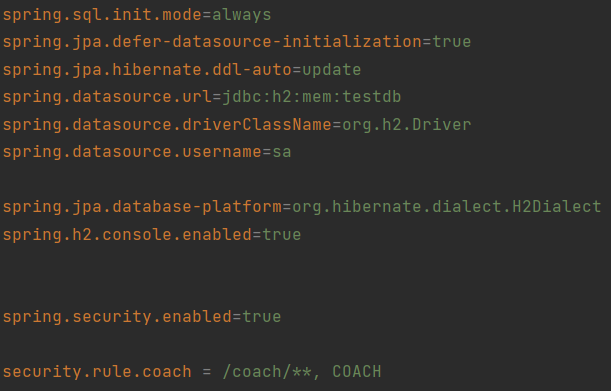
\includegraphics[scale=0.7]{./Slike/lokalno.png}
                      \centering
                      \caption{Konfiguracija postavki za pokretanje backenda lokalno}
                      \label{fig:promjene}
                \end{figure}

            {Za potrebe razvoja koristili smo se in-memory h2 bazom podataka. Aplikacija se pokreće na localhost:8080 portu. Ukoliko želimo prelgedavati stanje u bazi, koristimo URL: localhost:8080/h2-console. }
            \begin{figure}[H]
                      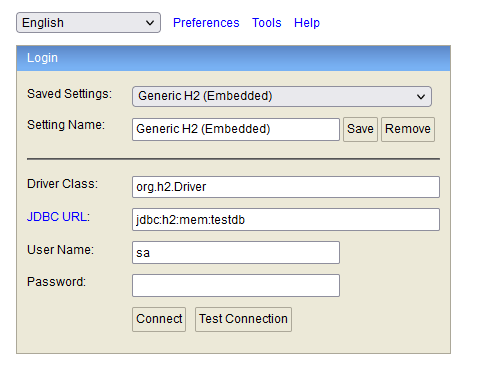
\includegraphics[scale=0.7]{./Slike/h2baza.png}
                      \centering
                      \caption{Konzola za in-memory bazu}
                      \label{fig:promjene}
                \end{figure}

            {Pokretanje frontenda obavlja se iz naredbenog retka. Najprije se pozicioniramo u direktorij sa package.json fileom (/group-fitness-planer/Frontend/groupfitnessui) i u njemu izvedemo naredbe:\\ 
            \textbf{npm install} \\
            koja instalira sve node module potrebne za pokretanje aplikacije, te \\
            \textbf{npm start} \\
            koja pokreće aplikaciju na localhost:8080 (namješteno tako da se front i back pokreću na istom portu kako bi mogli komunicirati). Stranica se ponovno učitava svakom spremljenom promjenom u kodu. 
            \\}
            
}
		
			%\textbf{\textit{dio 2. revizije}}\\
		
			 %\textit{U ovom poglavlju potrebno je dati upute za puštanje u pogon (engl. deployment) ostvarene aplikacije. Na primjer, za web aplikacije, opisati postupak kojim se od izvornog kôda dolazi do potpuno postavljene baze podataka i poslužitelja koji odgovara na upite korisnika. Za mobilnu aplikaciju, postupak kojim se aplikacija izgradi, te postavi na neku od trgovina. Za stolnu (engl. desktop) aplikaciju, postupak kojim se aplikacija instalira na računalo. Ukoliko mobilne i stolne aplikacije komuniciraju s poslužiteljem i/ili bazom podataka, opisati i postupak njihovog postavljanja. Pri izradi uputa preporučuje se \textbf{naglasiti korake instalacije uporabom natuknica} te koristiti što je više moguće \textbf{slike ekrana} (engl. screenshots) kako bi upute bile jasne i jednostavne za slijediti.}
			
			
			 %\textit{Dovršenu aplikaciju potrebno je pokrenuti na javno dostupnom poslužitelju. Studentima se preporuča korištenje neke od sljedećih besplatnih usluga: \href{https://aws.amazon.com/}{Amazon AWS}, \href{https://azure.microsoft.com/en-us/}{Microsoft Azure} ili \href{https://www.heroku.com/}{Heroku}. Mobilne aplikacije trebaju biti objavljene na F-Droid, Google Play ili Amazon App trgovini.}
			
			
			\eject 
	%\chapter{Zaključak i budući rad}
		
		%\textbf{\textit{dio 2. revizije}}\\
		
		{Primarni cilj ovog projekta bio je razviti aplikaciju koja omogućuje polaznicima treninga odabir treninga po terminu i tipu, koje korisnik može pohađati u skladu sa svojim slobodnim vremenom. Na taj način termini vježbanja prilagođavaju se slobodnom vremenu vježbača (polaznika), te su vježbači puno zadovoljniji jer mogu uložiti više pažnje vježbanju, i dobiti maksimalnu korist i dobrobit od usluga koje teretana, koja se koristi aplikacijom, pruža. \\}

        {Iz projektnog zadatka bilo je potrebno izlučiti funkcionalne i nefunkcionalne zahtjeve, konceptualno osmisliti, dokumentirati, a zatim i implementirati osmišljeno. Mentori ovog projekta ujedno su „glumili“ i klijente, pa smo komunikacijom s njima definirali koje funkcionalnosti žele vidjeti u aplikaciji, što ona mora sadržavati.  \\}

        {Provedba projekta bila je podijeljena u dva ciklusa. U prvom ciklusu oformili smo projektni tim, uspostavili kanale komunikacije, upoznali se sa zadatkom i krenuli u osmišljavanje rješenja zadatka. Inicijalne funkcionalnosti koje je naša aplikacija imala bili su prijava i registracija korisnika u sustav. Redovitim sastancima i komunikacijom preko društvenih mreža podijelili smo se u timove, zadužili se za pojedine zadatke i funkcionalnosti, te jasno definirali što koja funkcionalnost radi kako bismo svi imali jednaku ideju i razumjevanje zadaka. \\} 

        {U drugom ciklusu veći naglasak je bio na implementaciji same aplikacije. Dok smo se svi u prvom ciklusu „upoznavali“ i po prvi put susreli sa programskim alatima koje trebamo koristiti, u drugom ciklusu naglasak je bio na individualnom radu i programskoj implementaciji. Sve funkcionalnosti opisane obrascima uporabe su implementiranje, a one koje nisu opisane, nisu niti implementirane. \\}

        {Korist ovog projekta bila je prvenstveno edukacijska. Jako puno smo naučili o tehnologijama kojima smo implementirali aplikaciju, ali i o timskom radu, komunikaciji i dobili smo uvid od svojih mentora kako je raditi  takve projekte u pravim firmama za stvarne klijente. Iako smo se trudili implementirati sve željene funkcionalnosti, svjesni smo kako je potrebno još mnogo rada i vještine kako bi ona zaista bila na nivou na kakav su korisnici danas navikli. Trenutna verzija simbolizira prototip kojeg bilo koji član tima jednog dana može unaprjeđivati i usavršavati ukoliko bude imao interesa. Smatramo da je aplikacija korisna i primjenjiva svakom od nas jer se, kao i većina ljudi, brinemo o svome zdravlju, nastojimo baviti fizičkom aktivnosti i povremeno odlaziti u teretane, te se lako vidimo kako aplikaciju u budućnosti zaista i upotrebljavamo. \\}
		
		 %\textit{Potrebno je točno popisati funkcionalnosti koje nisu implementirane \\u ostvarenoj aplikaciji.}
		
		%\eject 
	\chapter*{Popis literature}
		\addcontentsline{toc}{chapter}{Popis literature}
	 	
 		\textbf{\textit{Kontinuirano osvježavanje}}
	
		\textit{Popisati sve reference i literaturu koja je pomogla pri ostvarivanju projekta.}
		
		
		\begin{enumerate}
			
			
			\item  Programsko inženjerstvo, FER ZEMRIS, \url{http://www.fer.hr/predmet/proinz}
			
			\item  I. Sommerville, "Software engineering", 8th ed, Addison Wesley, 2007.
			
			\item  T.C.Lethbridge, R.Langaniere, "Object-Oriented Software Engineering", 2nd ed. McGraw-Hill, 2005.
			
			\item  I. Marsic, Software engineering book``, Department of Electrical and Computer Engineering, Rutgers University, \url{http://www.ece.rutgers.edu/~marsic/books/SE}
			
			\item  The Unified Modeling Language, \url{https://www.uml-diagrams.org/}
			
			\item  Astah Community, \url{http://astah.net/editions/uml-new}
		\end{enumerate}
		
		 
	
	
	\begingroup
	\renewcommand*\listfigurename{Indeks slika i dijagrama}
	%\renewcommand*\listtablename{Indeks tablica}
	%\let\clearpage\relax
	\listoffigures
	%\vspace{10mm}
	%\listoftables
	\endgroup
	\addcontentsline{toc}{chapter}{Indeks slika i dijagrama}


	
	\eject 
		
	\chapter*{Dodatak: Prikaz aktivnosti grupe}
		\addcontentsline{toc}{chapter}{Dodatak: Prikaz aktivnosti grupe}
		
		\section*{Dnevnik sastajanja}
						
		\begin{packed_enum}
			\item  sastanak
			
			\item[] \begin{packed_item}

				\item Datum: 24. listopada 2022.
				\item Prisustvovali: Bruna Kaštela, Tomislav Kožul, Petar Lovrić, Damir Numić-Meša, Rujana Perić, Petra Renić, Nika Šljubura
				\item Teme sastanka: uvodni sastanak
				\begin{packed_item}
					\item  upoznavanje
					\item  određivanje kanala komunikacije
                    \item  odabir tehnologija
                    \item  raspodjela zaduženja unutar tima

				\end{packed_item}
			\end{packed_item}
			
			\item  sastanak
			\item[] \begin{packed_item}

				\item Datum: 3. studenoga 2022.
				\item Prisustvovali: Bruna Kaštela, Tomislav Kožul, Petar Lovrić, Damir Numić-Meša, Rujana Perić, Petra Renić, Nika Šljubura
				\item Teme sastanka: daljnji rad na projektu
				\begin{packed_item}

					\item  raspravljanje oko dodjeljenog zadatka
					\item  definiranje funkionalnih i nefunkcionalnih zahtjeva
                    \item  definiranje ostalih zahtjeva
                    \item  raspodjela pisanja dokumentacije
				\end{packed_item}
			\end{packed_item}
        \eject

			\item  sastanak
			\item[] \begin{packed_item}
				\item Datum: 10. studenoga 2022. 
				\item Prisustvovali: Bruna Kaštela, Tomislav Kožul, Petar Lovrić, Damir Numić-Meša, Rujana Perić, Petra Renić, Nika Šljubura
				\item Teme sastanka: daljnji rad na projektu
				\begin{packed_item}
					\item  kontrolna točka, prezentiranje dosad napravljenog
					\item  detaljna razrada svih Use caseova sustava
                    \item  razmjena informacija o tehnologijama
                    \item  raspodjela oko predstojećih zadataka

				\end{packed_item}
			\end{packed_item}

            \item  sastanak
			\item[] \begin{packed_item}
				\item Datum: 17. studenoga 2022. 
				\item Prisustvovali: Bruna Kaštela, Tomislav Kožul, Petar Lovrić, Damir Numić-Meša, Rujana Perić, Petra Renić, Nika Šljubura
				\item Teme sastanka: revizija prilikom prvog kolokviranja
				\begin{packed_item}
					\item  prezentiranje dosad napravljenog
					\item  testiranje postojećih funkcionalnosti
                    \item  diskusija o predaji prve inačice aplikacije

				\end{packed_item}
			\end{packed_item}

            \item  sastanak
			\item[] \begin{packed_item}
				\item Datum: 17. studenoga 2022. 
				\item Prisustvovali: Bruna Kaštela, Tomislav Kožul, Petar Lovrić, Damir Numić-Meša, Rujana Perić, Petra Renić, Nika Šljubura
				\item Teme sastanka: revizija prilikom prvog kolokviranja
				\begin{packed_item}
					\item  prezentiranje dosad napravljenog
					\item  testiranje postojećih funkcionalnosti
                    \item  diskusija o predaji prve inačice aplikacije

				\end{packed_item}
			\end{packed_item}

            \item  sastanak
			\item[] \begin{packed_item}
				\item Datum: 7. prosinca 2022. 
				\item Prisustvovali: Bruna Kaštela, Tomislav Kožul, Petar Lovrić, Damir Numić-Meša, Rujana Perić, Petra Renić, Nika Šljubura
				\item Teme sastanka: nastavak rada na projektu, ulazak u drugu fazu
				\begin{packed_item}
					\item  definiranje novih zadataka
					\item  podjela oko novih zadataka
                    \item  uvid u dosad napravljeno

				\end{packed_item}
			\end{packed_item}

            \item  sastanak
			\item[] \begin{packed_item}
				\item Datum: 17. prosinca 2022. 
				\item Prisustvovali: Bruna Kaštela, Tomislav Kožul, Petar Lovrić, Damir Numić-Meša, Rujana Perić, Petra Renić, Nika Šljubura
				\item Teme sastanka: nastavak rada na projektu
				\begin{packed_item}
					\item   kontrolna točka
                    \item  uvid u dosad napravljeno

				\end{packed_item}
			\end{packed_item}

            \item  sastanak
			\item[] \begin{packed_item}
				\item Datum: 3. siječnja 2023. 
				\item Prisustvovali: Bruna Kaštela, Tomislav Kožul, Petar Lovrić, Damir Numić-Meša, Rujana Perić, Petra Renić, Nika Šljubura
				\item Teme sastanka: nastavak rada na projektu
				\begin{packed_item}
					\item  kontrolna točka
                    \item  uvid u dosad napravljeno
                    \item  ulazak u završnu fazu projekta
				\end{packed_item}
			\end{packed_item}
			
		\end{packed_enum}
		
		\eject
		\section*{Tablica aktivnosti}
					
			\begin{longtblr}[
					label=none,
				]{
					vlines,hlines,
					width = \textwidth,
					colspec={X[7, l]X[1, c]X[1, c]X[1, c]X[1, c]X[1, c]X[1, c]X[1, c]}, 
					vline{1} = {1}{text=\clap{}},
					hline{1} = {1}{text=\clap{}},
					rowhead = 1,
				} 
				\multicolumn{1}{c|}{} & \multicolumn{1}{c|}{\rotatebox{90}{\textbf{Tomislav Kožul}}} & \multicolumn{1}{c|}{\rotatebox{90}{\textbf{Damir Numić-Meša }}} &	\multicolumn{1}{c|}{\rotatebox{90}{\textbf{Bruna Kaštela }}} & \multicolumn{1}{c|}{\rotatebox{90}{\textbf{Petar Lovrić }}} &	\multicolumn{1}{c|}{\rotatebox{90}{\textbf{Nika Šljubura }}} & \multicolumn{1}{c|}{\rotatebox{90}{\textbf{Petra Renić }}} &	\multicolumn{1}{c|}{\rotatebox{90}{\textbf{Rujana Perić}}} \\  
				Upravljanje projektom 		&  & 3 &  &  &  &  & \\ 
				Opis projektnog zadatka 	&  4  &  &  &  &  & \\ 
				
				Funkcionalni zahtjevi       &  &  &  &  & 2 &  &  \\ 
				Opis pojedinih obrazaca 	&  & 6 & 6 & 3 &  &  &  \\ 
				Dijagram obrazaca 			&  &  &  &  &  &  3  \\ 
				Sekvencijski dijagrami 		&  &  &  &  &  &  & 4  \\ 
				Opis ostalih zahtjeva 		& 1 &  &  &  &  &  &  \\ 

				Arhitektura i dizajn sustava	 &  &  5  &  &  &  &  &  \\ 
				Baza podataka				&  &  4  &  3  &  &  &   \\ 
				Dijagram razreda 			&  &  2  &  &  &  &   \\ 
				Dijagram stanja				&  &  & 1 &  &  &  &  \\ 
				Dijagram aktivnosti 		&  &  &  &  &  &  &2  \\ 
				Dijagram komponenti			&  &  &  &  &  &  &2  \\ 
				Korištene tehnologije i alati 		&  &  4  & 5 &  &  &  &  \\ 
				Ispitivanje programskog rješenja 	& 1 & 3 & 1 & 1 & 1 & 1 & 1  \\ 
				Dijagram razmještaja			&  &  &  &  &  &  &  \\ 
				Upute za puštanje u pogon 		&  & 3 &  &  &  &  & 1 \\  
				Dnevnik sastajanja 			&  &  &  &  &  &  & 2  \\ 
				Zaključak i budući rad 		&  &  &  &  &  &  &  \\  
				Popis literature 			&  &  &  &  &  &  &  \\  
				&  &  &  &  &  &  &  \\ \hline 
				\textit{front end} 				& 12 &  &  & 6 & 12 & 6 &  \\  
				\textit{izrada baze podataka} 		 			&  & 5 & 5 &  &  &  & \\  
				\textit{spajanje s bazom podataka} 							&  & 1 &  &  &  &  & 2  \\ 
				\textit{back end} 							&  &  10  & 6 &  &  &  & 4  \\  
				 							&  &  &  &  &  &  &\\ 
			\end{longtblr}
					
					
		\eject
		%\section*{Dijagrami pregleda promjena}
		
		%\textbf{\textit{dio 2. revizije}}\\
		
		%\textit{Prenijeti dijagram pregleda promjena nad datotekama projekta. Potrebno je na kraju projekta generirane grafove s gitlaba prenijeti u ovo poglavlje dokumentacije. Dijagrami za vlastiti projekt se mogu preuzeti s gitlab.com stranice, u izborniku Repository, pritiskom na stavku Contributors.}
		
	


\end{document} %naredbe i tekst nakon ove naredbe ne ulaze u izgrađen dokument 